\documentclass[a4paper]{report}
\usepackage[T1]{fontenc}
\usepackage[utf8]{inputenc}
\usepackage[english,italian]{babel}
\usepackage[a4paper,top=2cm,bottom=2cm,left=3cm,right=3cm,heightrounded,bindingoffset=5mm]{geometry}
\usepackage{graphicx}
\usepackage{subcaption}
\usepackage{float}
\usepackage{listings}
\usepackage{comment}
\usepackage{amsmath}
\usepackage{csvsimple}
\usepackage{placeins}
\usepackage[dvipsnames]{xcolor}
\usepackage{hyperref}
\usepackage{minted}
\usepackage{csquotes}
\usepackage{mathtools}
\usepackage{appendix}
\usepackage{amssymb}
\usepackage{algorithm}
\usepackage[rightComments=false,noEnd=false,beginComment=//~]{algpseudocodex}
\usepackage[skip=5pt plus1pt, indent=0pt]{parskip}

%\usemintedstyle{borland}
%\definecolor{bg}{rgb}{0.91,1,0.91} % light green
\definecolor{bg}{rgb}{0.95,0.95,0.95}   % light gray
\renewcommand{\theFancyVerbLine}{\textcolor[rgb]{0.5,0.5,0.5}{\footnotesize\arabic{FancyVerbLine}}}

\renewcommand\listingscaption{Listato}

\usepackage[]{biblatex} %Imports biblatex package
\addbibresource{bibliografia.bib} %Import the bibliography file

\makeatletter
\renewcommand*{\ALG@name}{Algoritmo}
\makeatother


\algrenewcommand\algorithmicforall{\textbf{for each}}


\begin{document}
	
	\title{
		
\includegraphics[width=35mm]{logo_UNIUD.png}\\[4mm]
		\LARGE{UNIVERSIT\'A DEGLI STUDI DI UDINE}\\[4mm]
		\LARGE{CORSO DI LAUREA MAGISTRALE IN INFORMATICA}\\[1cm]
		\LARGE{Progetto}\\[2mm]
		\Large{per il corso di}\\[2mm]
		\LARGE{Programmazione su Architetture Parallele}\\[4mm]
		\Large{A.A. 2023-2024}\\[1cm]
		\LARGE{Implementazione Parallela dell'algoritmo Push-Relabel \\per il problema Max-Flow/Min-Cut}
 		}
 	\author{Claudio Lanzaro \and Daniele Milo}
	\date{26 Settembre 2024}
	\maketitle
	
	\tableofcontents	
	
    \chapter{Introduzione}

    \section{Descrizione del progetto}
    \textcolor{red}{TODO}
    
    \section{Gruppo}
    Il progetto è stato svolto da un gruppo di due studenti composto da:
    
        \begin{center}
        \begin{tabular}{ccc}
        \textbf{Matricola} & \textbf{Cognome e Nome} & \textbf{Indirizzo Mail}\\[1ex]
        \hline \\
            142252 & Lanzaro Claudio & lanzaro.claudio@spes.uniud.it\\[1ex]	142387 & Milo Daniele & milo.daniele@spes.uniud.it\\[1ex]
        \end{tabular}
        \end{center}

    \section{Consegna}
    Il lavoro svolto viene consegnato in un archivio \textbf{.zip} contenente:
    \begin{itemize}
        \item ...
    \end{itemize}
    

    % Descrizione problema mincut (informale)
% descrizione formale
% reti di flusso (intro breve)
% collegamento con maxflow (teorema)
% algoritmi maxflow
% push-relabel (perché?) parallelizzabile meglio
% pseudo-codice e descrizione algoritmo (seriale)
% implementazione seriale ???


\chapter{Descrizione del problema}\label{chap:DescrizioneProblema}

    \section{Minimum Cut Set}
        Un \textit{taglio} $S$ di un grafo non orientato $G = (V,E)$ è un sottoinsieme proprio di $V$ ($S \in V$ e $S \neq \emptyset ,V$). 
        La dimensione del taglio $S$ è il numero di archi tra $S$ e il resto del grafo $V \setminus S$. 
        Se il grafo è pesato, allora la dimensione del taglio corrisponde alla somma dei pesi degli archi che collegano le due parti.
    
        Il taglio $S$ è detto \textit{minimo} se, tra tutti i tagli possibili all'interno del grafo $G$, è quello di dimensione minima.
        
        Trovare il taglio minimo di un grafo non orientato e pesato sugli archi è un problema algoritmico fondamentale.
        Le sue applicazioni sono varie in campi come il routing nelle reti di telecomunicazione, la progettazione di circuiti, l'ottimizzazione delle risorse e la segmentazione di immagini.

        \subsection{Definizione formale}
            Il problema del taglio minimo (anche detto \textit{Min Cut Problem}) è definito come segue:
    
            \textbf{Input:} un grafo non orientato $G = (V, E)$. Due vertici $s,t \in V$. Pesi $w_{ij} \ge 0$ per ogni arco $ij \in E$.
            
            \textbf{Goal:} trovare $S \in V$ tale che $s \in S, t \notin S$ e 
            
            \begin{equation}
                \sum_{\mathclap{\substack{ij \in E : \\ i\in S \land j \notin S}}}w(i,j)
            \end{equation}
    
            ha valore minimo. Un caso speciale si verifica quando $w_{ij} = 1$ per tutti gli archi $ij \in E$ e, quindi, siamo interessati a trovare un taglio di cardinalità minima \cite{Lancia2022}.
    
    \section{Maximum Flow Problem}

        Il \textit{Minimum Cut} si connette al problema del \textit{Maximum Flow} attraverso il teorema del max-flow/min-cut, il quale afferma che il valore del flusso massimo da $s$ a $t$ è uguale al peso del taglio minimo che separa $s$ da $t$ nel grafo. Quindi, risolvere il problema del \textit{Minimum Cut} può essere ricondotto a calcolare il flusso massimo attraverso il grafo.

        Il problema del massimo flusso è formalizzato come segue:
        
        \textbf{Input:} una rete di flusso $G = (V, A, k)$ con $k$ capacità degli archi. Due vertici $s,t \in V$.
        
        \textbf{Goal:} trovare un flusso $s$-$t$ di valore massimo.

    \section{Algoritmi}\label{sec:algoritmi}

        Per risolvere il problema del \textit{Minimum Cut} e del \textit{Maximum Flow}, sono stati sviluppati diversi algoritmi che sfruttano approcci diversi per migliorare l'efficienza e l'accuratezza nella risoluzione.
    
        Gli algoritmi per il \textit{Maximum Flow} sono tra i più studiati in informatica teorica e applicata, poiché risolvere questo problema consente di ottenere informazioni utili anche per il \textit{Minimum Cut}, grazie al teorema del max-flow/min-cut. Alcuni dei principali algoritmi sono:

        \begin{itemize}
            \item \textbf{Algoritmo di Ford-Fulkerson}: è uno degli approcci più classici per risolvere il problema del massimo flusso. L'algoritmo costruisce incrementi di flusso lungo percorsi migliorativi fino a quando non è più possibile trovare percorsi che aumentino il flusso totale. L'implementazione di base ha complessità $O(|E| \cdot f)$, dove $f$ è il valore del massimo flusso. Tuttavia, con l'uso della versione basata sull'algoritmo di Edmonds-Karp, che utilizza la ricerca in ampiezza (BFS) per trovare i percorsi migliorativi, la complessità diventa $O(|V| \cdot |E|^2)$.
            
            \item \textbf{Algoritmo di Push-Relabel}: invece di basarsi su percorsi migliorativi come Ford-Fulkerson, questo algoritmo si concentra su un nodo alla volta. La complessità è $O(|V|^2 \cdot |E|)$.
        \end{itemize}

        Grazie al teorema del max-flow/min-cut, risolvere il problema del \textit{Maximum Flow} consente anche di risolvere il problema del \textit{Minimum Cut}. Gli algoritmi di flusso massimo possono essere modificati per trovare direttamente il taglio minimo associato al flusso massimo. In particolare, al termine dell'algoritmo del massimo flusso, è possibile identificare il taglio minimo osservando i vertici raggiungibili dalla sorgente (o dal pozzo) nel grafo residuo. Per maggiori dettagli riguardo le reti di flusso si veda l'Appendice \ref{app:flownet}.
        
    \section{Algoritmo Push-Relabel}

        %Per questo progetto abbiamo deciso di trattare l'algoritmo Push-Relabel proposto da Goldberg, Tarjan et al. \cite{PushRelabel} in quanto è relativamente più facile da parallelizzare rispetto ad altri algoritmi basati su cammini aumentanti \cite{EfficientCUDA2012, EngineeringWorkload2024}.

        Per questo progetto abbiamo deciso di trattare l'algoritmo Push-Relabel proposto da Goldberg e Tarjan \cite{PushRelabel}, in quanto non solo ha la migliore complessità teorica e pratica, ma è anche particolarmente adatto alla parallelizzazione grazie alla sua struttura intrinseca e alla natura locale delle sue operazioni, risultando relativamente più facile da parallelizzare rispetto ad altri algoritmi basati su cammini aumentanti \cite{EngineeringWorkload2024, EfficientCUDA2012}.
        
        L'algoritmo, conosciuto anche come preflow-push algorithm, si concentra su operazioni locali per aggiustare il flusso \cite{EngineeringWorkload2024}.

        L'idea di base dell'algoritmo push-relabel è generare il maggior flusso possibile alla sorgente e gradualmente spingerlo verso il pozzo. Introduce il concetto di \textit{excess flow} (flusso in eccesso), che consente a un vertice di ricevere più flussi in ingresso; in altre parole, consente a un vertice di avere più flusso in entrata di quanto ne esca durante la procedura push-relabel, e tale vertice viene chiamato \textit{attivo}. Denotiamo con $e(v)$ il valore del flusso in eccesso sul vertice $v$. La procedura dell'algoritmo push-relabel consiste nel trovare i vertici attivi e applicare su di essi le operazioni di \textit{push} e \textit{relabel} fino a quando non rimangono più vertici attivi. Per trovare i vertici attivi iniziali, l'algoritmo spinge il maggiori quantitativo di flusso possibile dalla sorgente a tutti i vertici adiacenti, operazione chiamata \textit{preflow} (preflusso). Un'operazione di push poi forza un vertice attivo a scaricare il suo flusso in eccesso e lo spinge verso i suoi vicini in $G_f$ (grafo residuo). Per evitare infiniti push, l'algoritmo introduce anche la funzione altezza $h$ su ciascun vertice. Inizialmente, l'altezza della sorgente è $|V|$, mentre l'altezza dei vertici rimanenti è 0. L'algoritmo, poi, forza un vertice attivo $u$ a spingere il flusso verso il vertice $v$ solo se $h(u) = h(v) + 1$. Se nessun vertice vicino soddisfa il vincolo, il vertice attivo aggiornerà la sua altezza trovando l'altezza minima $h'$ dei suoi vicini e aggiornando $h(u) \leftarrow h' + 1$. Con l'operazione di relabel, l'altezza di un vertice attivo, che non può spingere il suo flusso in eccesso, aumenterà. Il vertice attivo verrà disattivato una volta che la sua altezza supererà $|V|$. L'intera procedura termina quando non ci sono più vertici attivi \cite{EngineeringWorkload2024}.

        \begin{algorithm}
            \caption{Funzione \textit{Init} per l'algoritmo push-relabel}\label{alg:cap}
            \begin{algorithmic}
            \ForAll{$(x,y) \in E$}
                \State $f(x,y) \gets 1$
                \State $f(y,x) \gets 0$
            \EndFor

            \ForAll{$x \in V \setminus \{s\}$}
                \State $e(x) \gets 0$
                \State $h(x) \gets 1$
            \EndFor
            
            \State $e(s) \gets \infty$
            \State $h(s) \gets |V|$
            
            \end{algorithmic}
        \end{algorithm}

        \begin{algorithm}
            \caption{Funzione \textit{discharge(x)}}
            \begin{algorithmic}
                \If {($\exists\ (x,y) \in E_f : h(x)=h(y)+1$}
                    \State $push(x,y)$
                \Else
                    \State $relabel(x)$
                \EndIf
            \end{algorithmic}
        \end{algorithm}

        \begin{algorithm}
            \caption{Funzione \textit{push(x, y)}}
            \begin{algorithmic}
                \State $\delta \gets min\{u_f(x,y),\ e(x)\}$
                \State $e(x) \gets e(x) - \delta$
                \State $e(y) \gets e(x) + \delta$
                \State $f(x,y) \gets f(x,y) - \delta$
                \State $f(y,x) \gets f(y,x) + \delta$
            \end{algorithmic}
        \end{algorithm}

        \begin{algorithm}
            \caption{Funzione \textit{relabel(x)}}
            \begin{algorithmic}
                \State $h(x) \gets min\{h[y]:(x,y) \in E_f \} + 1$
            \end{algorithmic}
        \end{algorithm}

        \begin{algorithm}
            \caption{Algoritmo \textit{push-relabel}}
            \begin{algorithmic}
                \State \textit{Init()}
                \State make set $S$ empty
                \State $S \gets s$
                \While {($S$ is not empty)}
                    \State $x \gets S.$pop()
                    \State \textit{discharge(x)}
                    \If {($x$ is active node)}
                        \State $S.$push($x$)
                    \EndIf
                \EndWhile
            \end{algorithmic}
        \end{algorithm}

        \begin{algorithm}
            \caption{Algoritmo \textit{findMinCutSet($G_f$,s)}}
            \begin{algorithmic}
                \ForAll{$v \in V$}
                    \State $visited[v] \gets false$
                \EndFor
                \State $visited[s] \gets true$
                \State make queue $Q$ with $s$
                \While{$Q \neq \emptyset$}
                    \State $u \gets Q$.front()
                    \State $Q$.pop()
                    \ForAll{$v$ adjacent to $u$} \qquad \Comment{$(v,u) \in E_f$}
                        \If{not $visited[v]$}
                            \State $visited[v] \gets true$
                            \State $Q$.push(v)
                        \EndIf
                    \EndFor
                \EndWhile
            \end{algorithmic}
        \end{algorithm}



    % intro:
    % partiti da implementazione seriale per avere baseline per confronto di performance
    % implementata prima versione parallela CUDA 
    % miglioramento versione parallela con rappresentazione BCSR
    % versione migliore con workbalance e approccio vertex centric

% versione seriale
    % pseudo codice
        % global relabel (euristica)
        
% prima versione parallela
    % pseudo codice
    % cooperative groups (perché? senza c'era cattiva sincronizzazione tra threads)
    % tentativi di miglioramento con mem pagelocked e mapped mem
    % dati rappresentati con matrice di adiacenza
    % test -> troppa memoria utilizzata 


% rappresentazione CSR (e BCSR) [Appendice B?]

% miglioramento prima versione con rappresentazione BCSR
    % inserire confronti di pezzi di codice tra le due versioni

% versione workbalanced con approccio vertex centric
    % problema risolto: prima ogni thread si occupava di un solo nodo (se nodo non attivo, thread "sprecato")
    % ora: prima si cercano i nodi attivi e poi si suddividono i thread in gruppi e ognuno si occupa di un nodo
    % approccio ideato da [paper]
    % pseudo codice
    
% parallelizzaione findMinCutSet con OpenMP

% dati in input
    % random graphs (generazione)
    % DIMACS
    % funzioni per la lettura

% test condotti
    % per variazione di numero di nodi (a densità costante)
    % per variazione di densità (a  numero di nodi costante)
    % su istanze verosimili (DIMACS)
    % misurazione dei tempi
    % salvataggio risultati
    % calcolo tempi medi 

\chapter{Implementazione e ottimizzazioni}

    In questo capitolo presentiamo il percorso seguito per lo sviluppo di diverse versioni di un algoritmo parallelo per il calcolo del taglio minimo in un grafo. Il punto di partenza è stato l'implementazione di un algoritmo seriale, utilizzato come baseline per il confronto delle performance. Successivamente, si è passati a una prima versione parallela basata su CUDA, con l'obiettivo di sfruttare il calcolo parallelo per migliorare l'efficienza.

    Dopo questa prima versione, è stato introdotto un miglioramento significativo attraverso l'uso della rappresentazione BCSR (Bidirectional Compressed Sparse Row), ottimizzata per ridurre il consumo di memoria e migliorare l'accesso ai dati. A seguire, ulteriori ottimizzazioni sono state implementate tramite un approccio work-balanced e vertex-centric, che hanno risolto il problema della scarsa efficienza dei thread inattivi, migliorando il bilanciamento del carico di lavoro tra i thread attivi. Questo approccio è stato proposto da un recente studio \cite{EngineeringWorkload2024} e si è dimostrato efficace nel massimizzare l'utilizzo delle risorse hardware.
    
    Infine, vengono presentati i dettagli dei test eseguiti utilizzando grafi generati casualmente e dataset standard in formato DIMACS. I test hanno valutato le prestazioni delle implementazioni in funzione del numero di nodi e della densità dei grafi, con un'analisi dettagliata dei tempi di esecuzione.


    \section{Versione seriale}

        La prima versione dell'algoritmo push-relabel implementata è stata quella seriale. Il codice sviluppato segue passo passo lo pseudocodice riportato nel Capitolo \ref{chap:DescrizioneProblema}.
        Le performance misurate sono apparse sin da subito scarse con tempi che crescevano esponenzialmente all'aumentare del numero di nodi del grafo in input.

        Le cause di questi risultati sono riconducibili in buona parte all'elevato numero di operazioni di relabel, molte delle quali inutili. 
        Per ovviare al problema, Goldberg e Tarjan hanno proposto un'euristica chiamata \textit{global relabeling} \cite{PushRelabel} che impedisce all'altezza dei nodi di aumentare velocemente e assegna ai nodi la minor altezza possibile.

        La tecnica di global relabeling prevede l'esecuzione di una Breadth First Search (BFS) all'indietro (partendo dal nodo sink) nel grafo residuo, assegnando ai nodi nuove altezze corrispondenti al livello di ciascun nodo nell'albero BFS. La BFS richiede un tempo lineare pari a $O(m + n)$. In genere, il global relabeling viene applicato una volta ogni $n$ operazioni di relabel. Questa euristica migliora notevolmente le prestazioni dell'algoritmo push-relabel.

        Questa euristica, riportata nell'Algoritmo \ref{alg:global-relabel}, è stata implementata in tutte le versioni parallele che verranno descritte in seguito in questo capitolo.

        \begin{algorithm}
            \caption{Euristica \textit{Global Relabeling}}\label{alg:global-relabel}
            \begin{algorithmic}
                \State make queue $Q$ empty 
                \ForAll{$v \in V$}
                    \State $scanned[v] \gets false$
                \EndFor
                \State $Q.$push($t$)
                \State $scanned[t] \gets true$
                \While{$Q \neq \emptyset $}
                    \State $x \gets Q.$pop()
                    \State $current \gets h(x)$
                    \State $current \gets current + 1$
                    \ForAll{$(y,x) \in E_f : y $ not scanned}
                        \State $h(y) \gets current$
                        \State $scanned[y] \gets true$
                        \State $Q.$pop()
                    \EndFor     
                \EndWhile
            \end{algorithmic}
        \end{algorithm}


    \section{Prima versione parallela}

        Nella versione parallelizzata dell'algoritmo push-relabel si assume che il numero di thread in esecuzione sia |V| e che ciascuno di essi gestisca esattamente un nodo del grafo, comprese tutte le operazioni di push e relabel su di esso. In alcuni casi, più nodi possono essere gestiti da un solo thread.

        Sia $x$ il thread in esecuzione che rappresenta il nodo $x \in V$. Ogni thread ha i seguenti attributi privati: 
        \begin{itemize}
        \item la variabile $e'$ che memorizza l'eccesso del nodo $x$;
        \item la variabile $h''$ che memorizza l'altezza del vicino $y$ di $x$ tale che $(x, y) \in E_f$;
        \item la variabile $h'$ che memorizza l'altezza del vicino $y'$ di $x$ con altezza minore.
        \end{itemize}
        
        Altre variabili sono condivise tra tutti i thread in esecuzione. Tra queste ci sono gli array che contengono gli eccessi ($e$) e le altezze dei nodi ($h$), le capacità residue degli archi ($c_f$) e una variabile $TotalExcess$ equivalente al valore del flusso uscente dal nodo sorgente.

        Tutti i thread in esecuzione hanno accesso alle variabili nella memoria globale, ma i loro compiti vengono eseguiti sequenzialmente grazie all'accesso atomico ai dati. L'ordine delle operazioni in questa sequenza non può essere previsto. Nonostante ciò, l'algoritmo può essere dimostrato corretto.

        Inizialmente, l'operazione di inizializzazione ($Init$) viene eseguita dall'host (Algoritmo \ref{alg:parallel-init}). Questo codice di inizializzazione è lo stesso della versione seriale dell'algoritmo push-relabel.
        
        Il corpo principale dell'algoritmo è controllato dall'host. Il thread host esegue un ciclo \verb|while| fino a quando il valore cumulativo degli eccessi memorizzati nella sorgente e nel pozzo raggiunge il valore di $TotalExcess$ (Algoritmo \ref{alg:parallel-main}). A questo punto, tutto il flusso valido arriva al pozzo, mentre il resto del flusso torna alla sorgente. Di conseguenza, l'eccesso nel pozzo è uguale al valore del flusso massimo.

        Nel primo passo del ciclo \verb|while|, il thread host copia le altezze dei nodi nel device e avvia il kernel push-relabel. Quando il controllo ritorna al thread host, il "flusso" calcolato e le altezze dei nodi vengono copiati nella memoria della CPU e viene eseguita l'operazione di global-relabel. 
        
        Nel kernel push-relabel (Algoritmo \ref{alg:parallel-pr-kernel}), per $CYCLE$ iterazioni (dove $CYCLE$ è una costante che abbiamo definito pari a $|V|$), il thread cerca il nodo vicino con altezza minore verso cui effettuare un'operazione di push o di relabel. 
        Il ciclo \verb|while| nel kernel, quindi, si interrompe dopo un numero di iterazioni definito da $CYCLE$ e non quando il suo nodo diventa inattivo.  

        Al momento dell'esecuzione del global-relabeling (Algoritmo \ref{alg:parallel-global-relabel}), poiché il ciclo \verb|while| del kernel può terminare in qualsiasi momento, può verificarsi che la proprietà di alcuni archi residui $(x, y) \in E_f$ venga violata, cioè $h(x) > h(y) + 1$. Pertanto, prima di calcolare le nuove altezze dei nodi con il global-relabeling, tutti gli archi che violano la proprietà vengono corretti tramite il push del flusso. Gli eccessi dei nodi che non sono raggiungibili dalla BFS all'indietro devono essere sottratti da $TotalExcess$ poiché rappresentano un eccesso accumulato che non raggiungerà mai il pozzo.

        
        \begin{algorithm}
            \caption{\textit{Init()}}\label{alg:parallel-init}
            \begin{algorithmic}
                \State $h(s) \gets |V|$
                \State $e(s) \gets 0$
                \ForAll{$(u,y) \in E$}
                    \State $c_f(x,y) \gets c_{xy}$
                    \State $c_f(y,x) \gets c_{yx}$
                \EndFor
                \ForAll{$(s,x) \in E$}
                    \State $c_f(s,x) \gets 0$
                    \State $c_f(x,s) \gets c_{xs} + c_{sx}$
                    \State $e(s) \gets c_{sx}$
                    \State $TotalExcess \gets TotalExcess + c_{sx}$
                \EndFor
            \end{algorithmic}
        \end{algorithm}

        \begin{algorithm}
            \caption{\textit{PushRelabelKernel()}}\label{alg:parallel-pr-kernel}
            \begin{algorithmic}
                \State $cycle =$ CYCLE
                \While{$cycle > 0$}
                    \If{$e(x) > 0$ and $h(x) < |V|$}
                        \State $e' \gets e(x)$
                        \State $h' \gets \infty$
                        \ForAll{$(x,y) \in E_f$}
                            \State $h'' \gets h(y)$
                            \If{$h'' < h'$}
                                \State $y' \gets y$
                                \State $h' \gets h''$
                            \EndIf
                        \EndFor
                        \If{$h(x) > h'$} \qquad \Comment{Thread performs PUSH}
                            \State $\delta \gets min\{e', c_f(x,y)\}$
                            \State AtomicAdd($c_f(y',x), \delta$)
                            \State AtomicSub($c_f(x,y'), \delta$)
                            \State AtomicAdd($e(y'), \delta$)
                            \State AtomicSub($e(x), \delta$)
                        \Else \qquad \Comment{Thread performs RELABEL}
                            \State $h(u) \gets h' + 1$
                        \EndIf
                    \EndIf
                    \State $cycle = cycle - 1$
                \EndWhile
            \end{algorithmic}
        \end{algorithm}
    
        \begin{algorithm}
            \caption{\textit{GlobalRelabel()}}\label{alg:parallel-global-relabel}
            \begin{algorithmic}
                \ForAll{$(x,y) \in E$}
                    \If{$h(x) > h(y) + 1$}
                        \State $e(x) \gets e(x) - c_f(x,y)$
                        \State $e(y) \gets e(y) + c_f(x,y)$
                        \State $c_f(y,x) \gets c_f(y,x) + c_f(x,y)$
                        \State $c_f(x,y) \gets 0$
                    \EndIf
                \EndFor
                \State do a backwards BFS from sink and assign the height function with each node’s BFS tree level
                \If{not all the nodes are scanned}
                    \ForAll{$x \in V$}
                        \If{$x$ is not scanned and not marked}
                            \State mark $x$
                            \State $TotalExcess \gets TotalExcess - e(x)$
                        \EndIf
                    \EndFor
                \EndIf
            \end{algorithmic}
        \end{algorithm}

        \begin{algorithm}
            \caption{\textit{Main()}}\label{alg:parallel-main}
            \begin{algorithmic}
                \State \textit{Init()}
                \State Copy $e$ and $c_f$ from the CPU's main memory to the CUDA device global memory
                \While{$e(s)+e(t) < TotalExcess$}
                    \State Copy $h$ from the CPU's main memory to the CUDA device global memory
                    \State \textit{PushRelabelKernel()}
                    \State Copy $e$, $c_f$ and $h$ from the CUDA device global memory to the CPU's main memory
                    \State \textit{GlobalRelabel()}
                \EndWhile
            \end{algorithmic}
        \end{algorithm}


        \subsection{Implementazione kernel Push-Relabel}

            \textbf{Nota:} tutti i nomi di funzioni che seguiranno fanno riferimento al codice consegnato.
            
            La funzione host \verb|pushRelabel| gestisce l'intero processo dell'algoritmo, eseguendo i seguenti passaggi:
            \begin{itemize}
                \item preflow iniziale dai nodi sorgente;
                \item trasferimento delle variabili necessarie sulla memoria device;
                \item lancio del kernel \verb|pushRelabelKernel| per eseguire il ciclo di push-relabel in parallelo;
                \item trasferimento delle variabili necessarie sulla memoria host;
                \item applicazione dell'operazione di global relabel per aggiornare le altezze dei nodi.
            \end{itemize}

            \subsubsection{Gestione della memoria}
                Le variabili principali, come le matrici di capacità (\verb|d_capacities|), flusso residuo (\verb|d_residual|), altezza dei nodi (\verb|d_height|) e flusso in eccesso (\verb|d_excess|), vengono allocate nella memoria globale della GPU. I dati vengono trasferiti dalla memoria host a quella device tramite \verb|cudaMemcpy| prima dell'esecuzione del kernel e successivamente copiati di nuovo alla memoria host per ulteriori elaborazioni.

            \subsubsection{Kernel}
                Il kernel viene eseguito tramite la funzione \verb|cudaLaunchCooperativeKernel|, che sfrutta i cooperative groups per migliorare l'efficienza del calcolo parallelo. Il numero di blocchi (\verb|num_blocks|) è determinato dal numero di streaming multiprocessors della GPU, con ciascun blocco composto da 256 thread (\verb|block_size|), per ottimizzare il parallelismo.

                Il kernel \verb|pushRelabelKernel| implementa in modo parallelo l'algoritmo push-relabel, gestendo i nodi che hanno un eccesso di flusso. Ogni thread della GPU è responsabile di uno o più nodi, permettendo all'algoritmo di scalare su grafi di grandi dimensioni (tecnica \textit{Grid-Stride loops}). 

                L'uso di cooperative groups consente ai thread di sincronizzarsi durante l'esecuzione del kernel. La funzione \verb|grid.sync()| garantisce che tutte le operazioni di push e relabel siano completate prima di iniziare il ciclo successivo, mantenendo la coerenza dei dati condivisi tra i thread. Il kernel si concentra sui nodi attivi (esclusi quelli sorgente e destinazione), eseguendo le operazioni di push o relabel.
            
                Le operazioni di push vengono eseguite tramite operazioni atomiche, utilizzando \verb|atomicAdd| e \verb|atomicSub| per aggiornare in sicurezza le matrici del flusso residuo e dell'eccesso. La sincronizzazione con \verb|grid.sync()| dopo ogni ciclo assicura che tutti i thread completino le loro operazioni prima di passare al ciclo successivo. Questo è fondamentale per mantenere la coerenza dei dati condivisi tra i thread.

            \subsubsection{Sincronizzazione e gestione errori}
                Dopo il lancio del kernel, \verb|cudaDeviceSynchronize| viene chiamato per assicurare il completamento di tutte le operazioni prima di proseguire. Eventuali errori durante l'esecuzione vengono rilevati con \verb|cudaGetLastError|, fornendo messaggi diagnostici in caso di fallimento.


        \subsection{Test e miglioramenti}

            Questa prima versione parallela è stata testata su un insieme di grafi generati casualmente. Durante la fase iniziale di testing, grazie all'uso del profiler \textit{nvprof}, abbiamo osservato che la maggior parte del tempo di esecuzione veniva impiegata nei trasferimenti di dati tra host e device. Per ridurre tali tempi, abbiamo sperimentato diverse ottimizzazioni, tra cui l'uso della memoria page-locked e l'integrazione della memoria page-locked con quella mapped. Tuttavia, entrambe le versioni non hanno prodotto i miglioramenti attesi, anzi, i tempi di esecuzione sono persino aumentati. Pertanto, siamo tornati alla versione iniziale.

            Inoltre, i test hanno evidenziato una limitazione significativa: i grafi utilizzabili come input non potevano avere dimensioni elevate, poiché la loro rappresentazione matriciale richiede uno spazio di memoria pari a $O(V^2)$.

            Per superare questo vincolo, le prossime implementazioni adotteranno una rappresentazione dei dati più compatta.
            

    \section{Seconda versione parallela}

        Le precedenti versioni dell'algoritmo utilizzavano una matrice di adiacenza per rappresentare il grafo in input e quello residuo. Usare questo tipo di rappresentazione è comodo e richiede meno tempo in alcune fase del processo come la ricerca del nodo vicino con altezza minima. Tuttavia, come constatato nei primi test condotti, la complessità in termini di spazio è $O(V^2)$ e in presenza di grafi sparsi, o non particolarmente densi, provoca uno spreco di memoria impedendo la scalabilità delle soluzioni implementate.

        Per ovviare al problema, nelle versioni seguenti abbiamo adottato una rappresentazione chiamata \textit{Bidirectional Compressed Sparse Representation} (BCSR).
        
        \subsection{Bidirectional Compressed Sparse Representation}

            La \textit{Bidirectional Compressed Sparse Representation} proposta da Hsieh et al. \cite{EngineeringWorkload2024} è una evoluzione della classica rappresentazione CSR (Compressed Sparse Row).
            
            Il formato CSR offre già un notevole risparmio di memoria quando i grafi da rappresentare sono sparsi ma ha un piccolo difetto: dato un nodo $u$, dopo aver trovare il vicino $v$ con altezza minima, l'algoritmo push-relabel richiede di trovare l'arco $(v,u)$ e questa operazione non è ottimizzata al meglio.

            Con la BCSR si vuole migliorare questo aspetto. In particolare, i vicini (sia entranti che uscenti) vengono raggruppati e la lista \textit{column} è ordinata in modo crescente per ID del nodo. Così facendo, si può utilizzare una binary search per la ricerca dei nodi e ottenere performance migliori.

            In Figura \ref{fig:BCSR-example} è riportato un esempio di grafo residuo rappresentato sia tramite matrice di adiacenza che tramite BCSR.

            \begin{figure}[h]
                \centering
                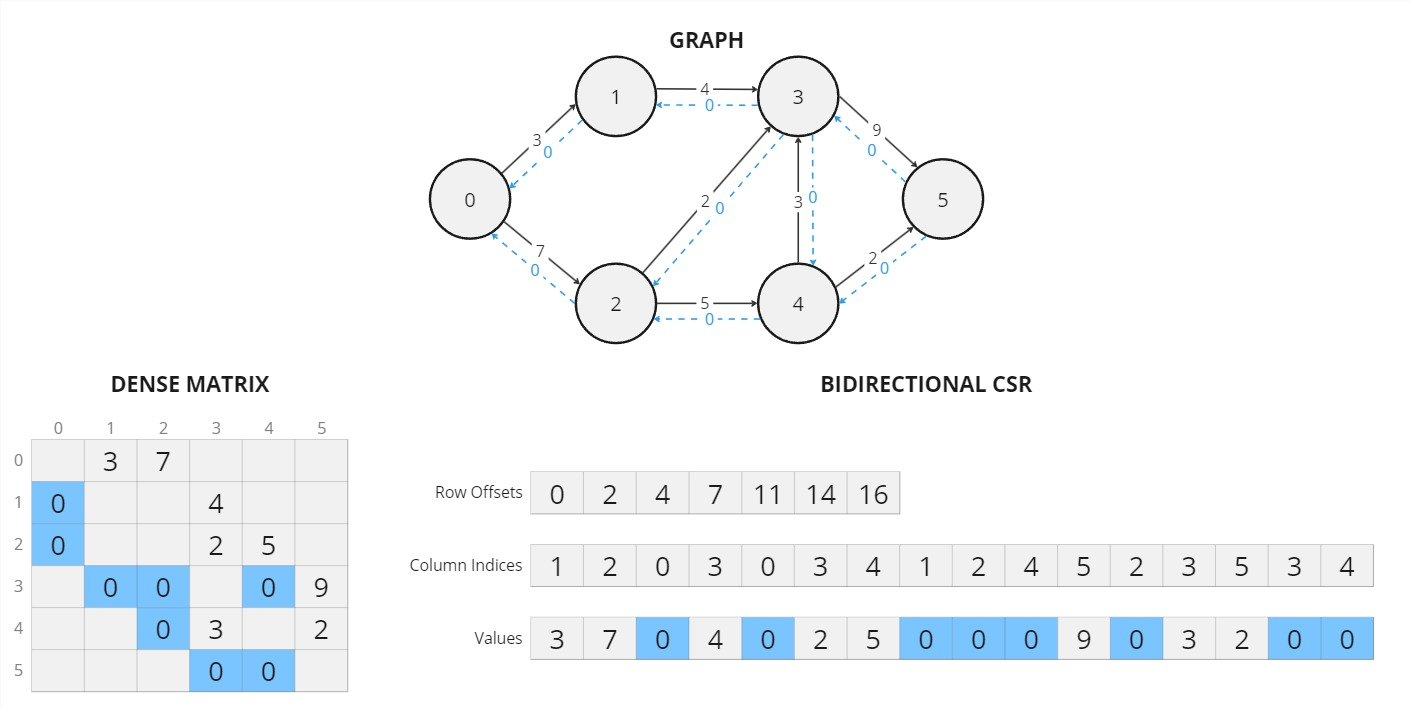
\includegraphics[width=1\linewidth]{images/bcsr-example.jpg}
                \caption{Matrice di adiacenza vs BCSR}
                \label{fig:BCSR-example}
            \end{figure}


            

        \subsection{Modifiche al codice}

            Con l'introduzione della nuova modalità di rappresentazione dei grafi, per adattare il codice della prima versione parallela, è stato sufficiente apportare delle piccole modifiche alle porzioni di codice che eseguivano accessi ai dati del grafo. Ad esempio, nei Listati \ref{code:matrix} e \ref{code:bcsr} sono confrontati gli accessi ai dati nella prima versione e quello nella seconda.
            
            \begin{listing}[h]
            \caption{Ricerca nodo vicino con matrice d'adiacenza}\label{code:matrix}
                \begin{minted}[linenos, numbersep=4pt, frame=leftline, framesep=8pt, bgcolor=bg]{cpp}
// Ricerca nodo adiacente con altezza minore
for(v = 0; v < V; v++){
    if(d_residual[u*V + v] > 0){
        h2 = d_height[v];
        ...
    }
}
                \end{minted}
            \end{listing}
            
            \begin{listing}[h]
                \caption{Ricerca nodo vicino con BCSR}\label{code:bcsr}
                \begin{minted}[linenos, numbersep=4pt, frame=leftline, framesep=8pt, bgcolor=bg]{cpp}
// Ricerca nodo adiacente con altezza minore
for(int i = d_offset[u]; i < d_offset[u+1]; i++){
    v = d_column[i];
    if(d_residual[i] > 0){
        h2 = d_height[v];
        ...
    }   
}
                \end{minted}
            \end{listing}

            Inoltre, dato che con BCSR trovare l'arco all'indietro non è immediato come nel caso con matrice di adiacenza, è stato necessario implementare un processo di ricerca apposito. Una prima soluzione è quella mostrata nel Listato \ref{code:linear-search}: per trovare l'arco all'indietro $(minV,u)$ occorre controllare per ogni vicino di $minV$ se quest'ultimo è $u$, in questo caso si salva l'indice $j$ dell'arco ricercato.
            
            \begin{listing}[h]
                \begin{minted}[linenos, numbersep=4pt, frame=leftline, framesep=8pt, bgcolor=bg]{cpp}
int backwardIdx = -1;

// Ricerca arco di ritorno
for(int j = d_offset[minV]; j < d_offset[minV+1]; j++){
    if(d_column[j] == u){
        backwardIdx = j;
        break;
    }
}
                \end{minted}
                \caption{Ricerca lineare}\label{code:linear-search}
            \end{listing}
            
            Successivamente, per sfruttare tutti i vantaggi che la BCSR offre, abbiamo sostituito questa porzione di codice con una equivalente che implementa la ricerca binaria (Listato \ref{code:binary-search}).
            
            \begin{listing}[ht]
                \begin{minted}[linenos, numbersep=4pt, frame=leftline, framesep=8pt, bgcolor=bg]{cpp}
int backwardIdx = -1;

// Ricerca arco di ritorno usando la ricerca binaria
int left = d_offset[minV];
int right = d_offset[minV + 1] - 1;

while (left <= right) {
    int mid = left + (right - left) / 2;
    if (d_column[mid] == u) {
        backwardIdx = mid;  // Arco di ritorno trovato
        break;
    } else if (d_column[mid] < u) {
        left = mid + 1;     // Cerca nella parte destra
    } else {
        right = mid - 1;    // Cerca nella parte sinistra
    }
}
                \end{minted}
                \caption{Ricerca binaria}\label{code:binary-search}
            \end{listing}
    
    \newpage
    \section{Terza versione parallela}

        Come ultima versione parallela, abbiamo voluto implementare la soluzione proposta da Hsieh et al. in \cite{EngineeringWorkload2024}. Si tratta di un approccio che combina l'utilizzo della rappresentazione BCSR e una distribuzione più equa del carico di lavoro tra i thread.

        Nelle versioni parallele analizzate finora è stato adottato un approccio \textit{thread-centric} in cui ogni thread gestiva le operazioni relative a un singolo nodo, indipendentemente dal fatto che fosse attivo o inattivo. Questo ha portato a uno spreco di risorse, poiché alcuni thread erano assegnati a nodi inattivi, mentre altri risultavano sovraccaricati, dovendo elaborare nodi con molti vicini e quindi richiedendo più lavoro.

        In questa versione si introduce, invece, un approccio \textit{vertex-centric} il quale si concentra esclusivamente sui nodi attivi distribuendo le risorse computazionali tra di essi. Hsieh et al. hanno chiamato questa versione \textit{workload-balanced push-relabel algorithm} \cite{EngineeringWorkload2024}.

        \subsection{Approccio vertex-centric}
            
            L'algoritmo inizia assegnando tutti i thread alla scansione dei vertici per individuare quelli attivi, che vengono poi aggiunti alla coda dei vertici attivi ($AVQ$). Questo approccio garantisce una distribuzione uniforme del carico di lavoro tra i thread durante la fase di identificazione dei vertici attivi. Inoltre, i vertici attivi vengono raggruppati all'interno dell'$AVQ$, consentendo di assegnare ad ogni nodo attivo un gruppo di thread (tile) per cercare il vicino con altezza minima. In questo modo, il tempo di ricerca viene ridotto.

            Nell'Algoritmo \ref{alg:workbalanced} è riportato lo pseudocodice che schematizza quanto appena detto. 
            
            Durante ciascuna iterazione, i vertici attivi vengono aggiunti alla coda AVQ tramite l'operazione AtomicAdd(). A questo punto, grazie all'inserimento di una sincronizzazione (grid.sync()), l'assegnazione dei thread può essere riorganizzata per ottimizzare la ricerca del vicino con altezza minima di ogni nodo attivo. Quando non ci sono più vertici attivi nella coda AVQ, il ciclo \verb|while| (Algoritmo \ref{alg:parallel-pr-kernel}) viene interrotto anticipatamente, evitando iterazioni non necessarie. Per migliorare l'efficienza, si usa un warp come tile che viene assegnato a ciascun vertice attivo per parallelizzare la ricerca del vicino minimo. La memorizzazione contigua dei vicini nella struttura BCSR permette di sfruttare la coalescenza della memoria, velocizzando il processo. Dopo aver identificato il vicino, il thread con $localIdx$ pari a 0 all'interno del warp esegue le operazioni di aggiornamento del grafo ("push" o "relabel").
            
            \begin{algorithm}
                \caption{\textit{PushRelabelKernel()}}\label{alg:workbalanced}
                \begin{algorithmic}
                    \State make a queue $avq$ empty
                    \State \Comment{Scanning active vertices}
                    \ForAll{$u \in V$}
                        \If{$e(u) > 0$ and $h(u) < |V|$}
                            \State $pos \gets$ AtomicAdd($avq, 1$)
                            \State $avq[pos] \gets u$  
                        \EndIf
                    \EndFor
                    \State grid.sync()
                    \State \Comment{Processing only active vertices}
                    \ForAll{$u \in avq$}
                        \State \Comment{Searching for min height neighbor of u}
                        \ForAll{$v \in neighbor(u)$}
                            \State $min =$ TiledSearchNeighbor()
                        \EndFor
                        \State tile.sync()
                        \State \Comment{Only one thread per tile computes push or relabel operations}
                        \If{$localIdx == 0$}
                            \If{$h(v) < h(min)$}
                                \State Push()
                            \Else
                                \State Relabel()
                            \EndIf
                        \EndIf
                    \EndFor
                \end{algorithmic}
            \end{algorithm}

            Nell'Algoritmo \ref{alg:tiled-search} viene descritto il processo di ricerca del vicino con altezza minima impiegando le tile. Si inizia con l'inizializzazione delle variabili necessarie e il calcolo del numero di iterazioni richieste per elaborare tutti i vicini del nodo utilizzando i thread contenuti nella tile. In questa fase preliminare si inizializza anche la memoria condivisa (shared memory), dove a ciascun thread viene assegnato lo spazio per tre interi: altezza, ID e indice del nodo vicino. Successivamente, per ogni iterazione prevista, si esaminano tutti i vicini, memorizzando solo le informazioni di quelli che soddisfano determinate condizioni.
            Una volta completata la scansione, viene effettuata una riduzione per ottenere le informazioni del nodo cercato. In seguito, uno dei thread della tile salva il risultato parziale prima di procedere all'iterazione successiva. Al termine di tutte le iterazioni, nelle variabili che contenevano i risultati parziali si troverà il risultato finale, che verrà infine restituito al chiamante.


            \begin{algorithm}
                \caption{\textit{TiledSearchNeighbor(tile, pos)}}\label{alg:tiled-search}
                \begin{algorithmic}
                    \State $idx \gets $ tile.thread\_rank() \Comment{thread index within the tile}
                    \State $tidx \gets threadIdx.x$ \Comment{thread index within the grid}
                    \State $u \gets avq[pos]$ \Comment{node whose neighbors will be scanned}
                    \State $degree \gets offset[u+1] - offset[u]$ \Comment{number of neighbors}
                    \State $numIters \gets \lceil degree / tileSize \rceil $
                    \State initialize variables $minH$ and $minV $ \Comment{to save intermediate and final result}
                    \State initialize shared memory variables $s\_height[tidx]$, $s\_vid[tidx]$, $s\_vidx[tidx]$
                    \For{$i = 0;$ $i < numIters;$ $i++$}
                        \State $vPos \gets offset[u] + i*tileSize + idx$
                        \State $v \gets column[vPos]$    
                        \If{$flows[vPos] > 0$ and $v \neq source$}
                            \State $s\_height[tidx] \gets d\_height[v]$
                            \State $s\_vid[tidx] \gets v$
                            \State $s\_vidx[tidx] \gets vPos$
                        \EndIf
                        \State tile.sync()
                        \State \Comment{Parallel reduction over shared memory values}
                        \For{$s = tile.size() / 2; s > 0; s >>= 1$}
                            \If{$idx < s$}
                                \If{$s\_height[tidx + s] < s\_height[tidx]$}
                                    \State $s\_height[tidx] \gets d\_height[tidx + s]$
                                    \State $s\_vid[tidx] \gets s\_vid[tidx + s]$
                                    \State $s\_vidx[tidx] \gets s\_vidx[tidx+ s]$    
                                \EndIf
                            \EndIf
                            \State tile.sync()
                        \EndFor
                        \State tile.sync()
                        \State \Comment{Only one thread updates the result of the current iteration}
                        \If{$idx == 0$}
                            \If{$minH > s\_height[tidx]$}
                                \State $minH = s\_height[tidx]$
                                \State $minV = s\_vid[tidx]$
                            \EndIf
                        \EndIf
                        \State tile.sync()
                        \State reset variables for next iteration
                        \State tile.sync()
                    \EndFor
                    \State tile.sync()
                    \State \Return $minV$
                \end{algorithmic}
            \end{algorithm}

            Un'ultima sostanziale differenza rispetto alle versioni precedenti è l'implementazione in CUDA anche della procedura di global-relabeling. La struttura del codice è molto simile a quella vista nelle precedenti versioni.     

    \newpage

    \section{Parallelizzazione ricerca del taglio minimo}

        Come anticipato nella Sezione \ref{sec:algoritmi}, al termine dell'esecuzione dell'algoritmo push-relabel, quello che si può ottenere immediatamente è il valore del massimo flusso. Per ottenere il minimum cutset, invece, occorre effettuare una visita in ampiezza (BFS) a partire da nodo pozzo (\textit{sink}). Nello specifico, l'insieme di taglio minimo sarà composto da tutti i nodi $v$ tali per cui esiste un cammino $v \xrightarrow{}^* sink$.

        Inizialmente, è stata implementata una versione seriale (\verb|findMinCutSetFromSink()|) che veniva eseguita sul grafo residuo restituito dall'algoritmo push-relabel. Durante i test, però, abbiamo riscontrato che la ricerca del minimum cutset impiegava, nel caso peggiore provato, decine di minuti rispetto ai pochi secondi impiegato da push-relabel.

        Vista tale differenza, abbiamo pensato di applicare delle ottimizzazioni tra cui la parallelizzazione tramite OpenMP. Di seguito descriveremo 3 versioni: quella seriale, quella parallela su matrice di adiacenza e quella parallela su rappresentazione BCSR.
        Ognuna di queste implementazioni è stata utilizzata assieme alle versioni opportune dell'algoritmo push-relabel.

        \subsection{Versione seriale}

            Questa versione è stata la prima implementata e quella che ha avuto le performance peggiori. Si tratta del punto di partenza da cui abbiamo sviluppato le versioni successive.
            Nel Listato \ref{code:mincut-serial} riportiamo il codice della funzione.

            \begin{listing}[ht]
            \begin{minted}[linenos, numbersep=4pt, frame=leftline, framesep=8pt, bgcolor=bg]{cpp}
std::vector<int> findMinCutSetFromSink(int V, int sink, int *offset, 
                                        int *column, int *forwardFlow){
    std::vector<int> minCutSet;
    std::queue<int> q;
    std::vector<bool> visited(V, false);

    // BFS per trovare il taglio minimo a partire dal nodo sink
    minCutSet.push_back(sink);
    q.push(sink);
    visited[sink] = true;

    while (!q.empty()) {
        int u = q.front();
        q.pop();

        // Scansione dei vicini di u che hanno flusso verso u
        for (int v = 0; v < V; v++) {
            for (int i = offset[v]; i < offset[v+1]; i++) {
                if(column[i] == u && forwardFlow[i] > 0 && !visited[v]) {
                    minCutSet.push_back(v);
                    q.push(v);
                    visited[v] = true;
                }
            }    
        }
    }

    return minCutSet;
}
            \end{minted}
            \caption{findMinCutSetFromSink - implementazione seriale}\label{code:mincut-serial}
            \end{listing}

        \subsection{Versione parallela su matrice di adiacenza}

            A partire dalla versione appena vista, abbiamo:
            \begin{itemize}
                \item sostituito la coda $q$ per memorizzare i nodi della frontiera con un vettore \textit{vertexList};
                \item distribuito i nodi della frontiera su più thread;
                \item introdotto delle strutture locali ai thread per ridurre gli accessi concorrenti;
                \item protetto la lettura dell'attributo \textit{visited} del nodo per evitare letture errate.
            \end{itemize}

            Per la distribuzione delle iterazioni del ciclo \verb|for| tra i thread, abbiamo provato diverse tecniche di schedulazione, quella migliore è risultata essere \verb|schedule(dynamic)|.

            La lettura di \verb|visited(v)| è stata inserita all'interno di una sezione critica per evitare race condition. Senza questa protezione, poteva verificarsi che un thread leggesse il valore \verb|false| per un nodo subito prima che un altro thread aggiornasse lo stesso valore a \verb|true|. Questa situazione avrebbe causato l'inserimento di duplicati dello stesso nodo nell'insieme del minimum cutset finale. La regione critica garantisce che l'accesso a \verb|visited(v)| avvenga in modo sicuro e sincronizzato tra i thread, prevenendo tali inconsistenze.
            
            Nel Listato \ref{code:mincut-parallel-adj} è riportato il codice completo.

            \begin{listing}
            \begin{minted}[linenos, numbersep=4pt, frame=leftline, framesep=8pt, bgcolor=bg]{cpp}
std::vector<int> findMinCutSetFromSinkOMP(int n, int t, int *residual){
    std::vector<int> minCutSet;
    std::vector<int> vertexList;
    std::vector<bool> visited(n, false);

    minCutSet.push_back(t);
    vertexList.push_back(t);
    visited[t] = true;

    while (!vertexList.empty()) {
        std::vector<int> newVertexList;
        
        #pragma omp parallel
        {
            std::vector<int> localVertexList;
            std::vector<int> localMinCutSet;

            #pragma omp for nowait schedule(dynamic)
            for (int i = 0; i < vertexList.size(); i++) {
                int u = vertexList[i];

                for (int v = 0; v < n; v++) {
                    bool shouldAdd = false;

                    #pragma omp critical (checkVisited)
                    {
                        if (!visited[v] && residual[v*n + u] > 0) {                         
                            visited[v] = true;
                            shouldAdd = true;
                        }
                    }

                    if(shouldAdd){
                        localMinCutSet.push_back(v);
                        localVertexList.push_back(v);
                    }
                }
            }

            #pragma omp critical (insert)
            {
                minCutSet.insert(minCutSet.end(), 
                    localMinCutSet.begin(), localMinCutSet.end());
                newVertexList.insert(newVertexList.end(), 
                    localVertexList.begin(), localVertexList.end());
            }
        }
        vertexList = newVertexList;
    }

    return minCutSet;
}
            \end{minted}
            \caption{findMinCutSetFromSinkOMP - implementazione parallela su matrice di adiacenza}\label{code:mincut-parallel-adj}
            \end{listing}
            
            
        \subsection{Versione parallela su rappresentazione BCSR}
     
            Per i dati rappresentati tramite il formato BCSR, l'approccio adottato è stato leggermente diverso. A causa della particolare struttura di questa rappresentazione, come già accennato, la ricerca dei nodi $v$, dato $u$, tali per cui esiste un arco ($v,u$) risulta più onerosa in termini computazionali rispetto al caso della matrice di adiacenza.
            
            Per ovviare a questo problema, tra le soluzioni analizzate, la più efficace è risultata essere quella illustrata nel Listato \ref{code:mincut-parallel-bcsr}. In questo caso, prima di iniziare la ricerca a partire dal \textit{sink}, viene calcolato il grafo residuo trasposto. Questo permette di evitare il problema della ricerca degli archi entranti, poiché una volta trasposto il grafo, sarà sufficiente seguire gli archi uscenti da ogni nodo incontrato durante la visita. 
            
            A parte questa modifica, il resto della procedura segue la stessa logica della versione basata sulla matrice di adiacenza, con alcuni adattamenti necessari per gestire la lettura dei dati secondo la struttura del formato BCSR.
            

        \begin{listing}
        \begin{minted}[linenos, numbersep=4pt, frame=leftline, framesep=8pt, bgcolor=bg, fontsize=\small]{cpp}
std::vector<int> findMinCutSetFromSinkOMP(int V, int E, int sink, 
                                int *offset, int *column, int *forwardFlow){
    int *t_offset = (int*)malloc((V+1)*sizeof(int));
    int *t_column = (int*)malloc(E*sizeof(int));
    int *t_forwardFlow = (int*)malloc(E*sizeof(int));
    for(int i = 0; i < V+1; i++){
        t_offset[i] = 0;
    }
    for(int i = 0; i < E; i++){
        t_column[i]= 0;
        t_forwardFlow[i] = 0;
    }
    
    computeTranspose(V, E, offset, column, forwardFlow, t_offset, 
                        t_column, t_forwardFlow);
    
    std::vector<int> minCutSet;
    std::vector<int> vertexList;
    bool *visited = (bool*)malloc(V*sizeof(bool));
    for(int i = 0; i < V; i++) {
        visited[i] = false;
    }
    minCutSet.push_back(sink);
    vertexList.push_back(sink);
    visited[sink] = true;
    while (!vertexList.empty()) {
        std::vector<int> newVertexList;      
        #pragma omp parallel
        {
            std::vector<int> localVertexList;
            std::vector<int> localMinCutSet;   
            #pragma omp for nowait schedule(dynamic)
            for (int i = 0; i < vertexList.size(); i++) {
                int u = vertexList[i];            
                for (int j = t_offset[u]; j < t_offset[u+1]; j++) {
                    int v = t_column[j];
                    bool shouldAdd = false;
                    #pragma omp critical (checkVisited)
                    {
                        if(!visited[v] && t_forwardFlow[j] > 0) {
                            visited[v] = true;
                            shouldAdd = true;
                        }
                    }   
                    if(shouldAdd) {
                        localMinCutSet.push_back(v);
                        localVertexList.push_back(v);
                    }
                }
            }
            #pragma omp critical (insert)
            {
                minCutSet.insert(minCutSet.end(), 
                        localMinCutSet.begin(), localMinCutSet.end());
                newVertexList.insert(newVertexList.end(), 
                        localVertexList.begin(), localVertexList.end());
            }
        }
        vertexList = newVertexList;
    }
    return minCutSet;
}
        \end{minted}
        \caption{findMinCutSetFromSinkOMP - implementazione parallela su rappresentazione BCSR}\label{code:mincut-parallel-bcsr}
        \end{listing}
    
    \newpage
    
    \section{Test e analisi delle performance}

        In ogni fase dello sviluppo delle varie versioni sono stati condotti dei test per verificare la correttezza del codice, individuare le parti da ottimizzare e confrontare le versioni finali per decretarne la migliore.
        In questa sezione descriveremo i dati utilizzati come input, le tecniche di misurazione dei tempi di esecuzione e gli strumenti per la visualizzazione dei dati ottenuti.

        \subsection{Dati di input}

            Durante lo svolgimento dei test sono stati impiegati 3 diversi gruppi di istanze di grafi:
            \begin{itemize}
                \item grafi generati casualmente con numero di nodi crescente e densità costante per misurare i tempi di esecuzione all'aumentare della dimensione dell'input;
                \item grafi generati casualmente con numero di nodi costante e densità crescente per confrontare le performance dei due tipi di rappresentazione dei grafi;
                \item grafi reperiti da un dataset online per testare gli algoritmi su istanza reali.
            \end{itemize}

            \subsubsection*{Generazione grafi casuali}

                Per la generazione dei grafi casuali abbiamo scritto un breve jupyter notebook in python e sfruttato alcune funzionalità della libreria \textit{networkx}.
                In particolare, è stata implementata la funzione \verb|generate_random_graph| (Listato \ref{code:generate-random-graph}), la quale utilizza il modello di grafi casuali Erdős-Rényi con una probabilità \textit{p} di creare un arco tra ciascuna coppia di nodi. I parametri di input per la funzione includono:
                \begin{itemize}
                    \item \verb|n|, il numero di nodi nel grafo;
                    \item \verb|p|, la probabilità con cui ogni arco viene creato tra due nodi;
                    \item \verb|min_capacity| e \verb|max_capacity|, i limiti inferiore e superiore per la capacità degli archi;
                    \item \verb|directed|, un parametro booleano che determina se il grafo sarà diretto o non diretto.
                \end{itemize}
                
                L'esecuzione della funzione genera un grafo con capacità casuali assegnate ad ogni arco. Un aspetto cruciale della generazione dei grafi è la connettività: per ogni istanza generata ci siamo assicurati che fosse connessa.

                I grafi indiretti sono stati generati tali ma durante la fase di scrittura su file sono stati simulati come diretti, duplicando ogni arco in entrambe le direzioni. Questo è stato fatto per far funzionare correttamente l'algoritmo push-relabel.
                
                Per il primo gruppo di grafi (nodi crescenti e densità costante) come valore di densità abbiamo scelto $p = 2(log(n)/n)$ poiché, secondo la teoria, la probabilità che un Erdős-Rényi random graph sia connesso è molto alta quando $p > log(n)/n$. Per quanto riguarda il numero di nodi, abbiamo scelto valori di $n$ fino a 100mila.

                Per il secondo gruppo, invece, i valori scelti sono stati $n = 1000$ e $p \in [0,1]$ con passo $0.1$.

                \begin{listing}[ht]
                \begin{minted}[linenos, numbersep=4pt, frame=leftline, framesep=8pt, bgcolor=bg]{python}
def generate_random_graph(n, p, min_capacity, max_capacity, directed=False):
    G = nx.gnp_random_graph(n, p, directed=directed, seed=7)

    for edge in G.edges:
        capacity = random.randint(min_capacity, max_capacity)
        G.edges[edge]['capacity'] = capacity
    
    return G
                \end{minted}
                \caption{Funzione per generare un grafo casuale con il modello Erdős-Rényi}\label{code:generate-random-graph}
                \end{listing}

                Una volta ottenuto il grafo generato, abbiamo scelto di salvarlo in un file di testo seguendo il formato:
                \begin{itemize}
                    \item una riga per indicare il numero di nodi presenti (es. \verb|n 500| indica 500 nodi con ID da 0 a 499);
                    \item una riga per ogni arco e la relativa capacità (es. \verb|e 1 2 5| indica arco da nodo 1 a nodo 2 con capacità 5).
                \end{itemize}
            

            \subsubsection*{Grafi da dataset online}

                I dati relativi al terzo gruppo di istanze è stato reperito al link \url{https://vision.cs.uwaterloo.ca/data/maxflow}. Si tratta di una pagina web in cui sono presenti molte istanze di grafi pesati raggruppati in dataset. Il dataset che abbiamo utilizzato per i test è chiamato \textit{BVZ-tsukuba}.

                I grafi sono salvati nel formato standard DIMACS, una sua descrizione è reperibile alla pagina \url{https://lpsolve.sourceforge.net/5.5/DIMACS_maxf.htm}.


            \subsubsection*{Lettura grafi da file}

                Come si può evincere da quanto appena detto, essendo presenti due formati di file in input, è stato necessario implementare anche due funzioni C++ per il caricamento dei dati prima dell'esecuzione dell'algoritmo push-relabel.

                La scelta di quale metodo chiamare è fatta in automatico sulla base dell'estensione del file passato al programma. Infatti, i grafi generati casualmente sono salvati in file \verb|.txt| mentre i file in formato DIMACS hanno estensione \verb|.max|.

            
        \subsection{Misurazione tempi}

            Per tutte le versioni dell'algoritmo implementate abbiamo misurato il tempo di inizializzazione (creazione e popolamento delle strutture dati e eventuali trasferimenti al device), tempo di esecuzione (dell'intero algoritmo push-relabel) e tempo totale (somma dei precedenti).

            \subsubsection*{Versione seriale}
            
                Nella implementazione seriale, per la rilevazione dei tempi, abbiamo utilizzato le funzioni della libreria \verb|chrono|. Nel Listato \ref{code:tempi-seriali} è riportato uno schema semplificato di come la misurazione è avvenuta.

                \begin{listing}[ht]
                \begin{minted}[linenos, numbersep=4pt, frame=leftline, framesep=8pt, bgcolor=bg]{cpp}
const auto start = chrono::high_resolution_clock::now();

[inizializzazione]

const auto endInitialization = chrono::high_resolution_clock::now();

[Esecuzione algoritmo push-relabel]

const auto end = chrono::high_resolution_clock::now();

double initializationTime = chrono::duration_cast<chrono::microseconds>
                                (endInitialization - start).count()/1000.0;
double executionTime = chrono::duration_cast<chrono::microseconds>
                                (end - endInitialization).count()/1000.0;
double totalTime = chrono::duration_cast<chrono::microseconds>
                                (end - start).count()/1000.0;


                \end{minted}
                \caption{Schema misurazione tempi (versione seriale)}\label{code:tempi-seriali}
                \end{listing}   

            \subsubsection*{Versioni parallele}
            
                Nelle implementazioni parallele, la misurazione dei tempi è avvenuta tramite i \verb|cudaEvent|. Nel Listato \ref{code:tempi-paralleli} è riportato uno schema esemplificativo.

                \begin{listing}[ht]
                \begin{minted}[linenos, numbersep=4pt, frame=leftline, framesep=8pt, bgcolor=bg]{cpp}
//Dichiarazione degli eventi per la misurazione del tempo
cudaEvent_t startEvent, endInitializationEvent, endEvent;
cudaEventCreate(&startEvent);
cudaEventCreate(&endInitializationEvent);
cudaEventCreate(&endEvent);

...

// Primo evento per la misurazione del tempo
cudaEventRecord(startEvent, 0);

[inizializzazione]

// Secondo evento per la misurazione del tempo
cudaEventRecord(endInitializationEvent, 0);

[Esecuzione algoritmo push-relabel]

// Terzo evento per la misurazione del tempo
cudaEventRecord(endEvent, 0);

// Attendo la fine dell'evento endEvent
cudaEventSynchronize(endEvent);

// Misurazione del tempo
float initializationTime = 0.0f;
float executionTime = 0.0f;
float totalTime = 0.0f;
cudaEventElapsedTime(&initializationTime, startEvent, endInitializationEvent);
cudaEventElapsedTime(&executionTime, endInitializationEvent, endEvent);
cudaEventElapsedTime(&totalTime, startEvent, endEvent);

// Distruzione degli eventi
cudaEventDestroy(startEvent);
cudaEventDestroy(endInitializationEvent);
cudaEventDestroy(endEvent);
                \end{minted}
                \caption{Schema misurazione tempi (versione parallela)}\label{code:tempi-paralleli}
                \end{listing}            

    \newpage
     
    \subsection{Esecuzione e analisi}

        Tutti i test eseguiti hanno prodotto dei risultati che sono stati salvati in opportuni file in formato JSON.
        Ognuno di essi conteneva:
        \begin{itemize}
            \item valore del massimo flusso;
            \item insieme dei nodi del minimum cutset;
            \item tempo di inizializzazione;
            \item tempo di esecuzione;
            \item tempo totale;
            \item numero di nodi del grafo;
            \item numero di archi.
        \end{itemize}

        Tutti questi file sono stati poi analizzati tramite un jupyter notebook in python per generare dei grafici che saranno mostrati nel Capitolo \ref{chap:Risultati}.

        Per garantire risultati più affidabili ed eliminare possibili interferenze che avrebbero potuto influenzare i risultati, ciascun test è stato eseguito 10 volte e successivamente è stata calcolata la media dei tempi registrati. 
        
        Inoltre, tutte le sessioni di test sono avvenute sulla macchina \textit{CUDA-srv} messa a disposizione dall'università con le seguenti caratteristiche:
        \begin{itemize}
            \item Intel Xeon W-3323 CPU @ 3.50GHz
            \item RAM 64GB
            \item Nvidia GeForce RTX 2080 Ti
        \end{itemize}



    % Risultati per test a grafo crescente in numero di nodi
    % tutte le versioni sia su diretti che indiretti
        % grafici confronto
        % commenti
    
% Risultati per test a grafo con densità crescente
    % grafico
    % osservazioni e possibii spiegazioni
        % con matrice tempo costante perché ...
        % con BCSR tempo crescente con densità perché ...
        % per densità elevate stessi tempi
        % linea viola bcsr senza ottimizzazioni work balance (inutile)
        


\chapter{Risultati}\label{chap:Risultati}

    In questo capitolo verranno discussi i principali risultati riscontrati durante la fase di testing. 

    Per facilitare la lettura dei grafici, si ricorda che:
    \begin{description}
        \item[{\color{blue}serial}] è la versione seriale, la prima implementata;
        \item[{\color{red}parallel}] è la prima versione parallela, i grafi sono rappresentati tramite matrice di adiacenza;
        \item[{\color{violet}parallelbcsrtc}] è la seconda versione parallela, molto simile alla precedente, viene adattata per la rappresentazione BCSR includendo le ottimizzazioni che quest'ultima consente;
        \item[{\color{YellowOrange}parallelbcsrvc}] è l'ultima versione implementata, la versione \textit{work balanced}, e applica alla versione precedente diverse ottimizzazioni per sfruttare al massimo le risorse computazionali.
    \end{description}

    Nella prima parte metteremo a confronto le varie implementazioni su input in cui il numero di nodi è variabile e la densità è costante. 
    Viceversa, nella seconda parte analizzeremo come la variazione di densità influisce sui tempi di esecuzione.

    \section{Risultati per quantità nodi variabile}

        Di seguito sono riportati due grafici che mettono a confronto le diverse implementazioni sia nel caso di grafi diretti (Figura \ref{fig:exec-time-dir}) che in quello di grafi indiretti (Figura \ref{fig:exec-time-undir}). I grafici rappresentano esclusivamente i tempi di esecuzione dell'algoritmo, sono esclusi quindi i tempi di inizializzazione e salvataggio dei risultati.

        I valori di tutti gli assi sono espressi in scala logaritmica. Altrimenti, vista la grande differenza tra i valori, alcune linee risulterebbero appiattite e sovrapposte, rendendo difficile l'analisi dei risultati.

        Sulle ordinate sono riportati i tempi espressi in millisecondi mentre sulle ascisse il numero di nodi.

        Prima di passare alle osservazioni sui grafici, facciamo notare che non tutte le versioni sono state testate su tutte le istanze a disposizione per i seguenti motivi:
        \begin{itemize}
            \item la versione seriale è risultata essere talmente inefficiente (in termini di tempo) da consentirne l'esecuzione solamente con piccole istanze;
            \item la prima versione parallela, usando la matrice di adiacenza come metodo di rappresentazione dei dati, è risultata limitata nell'utilizzo della memoria al punto da renderne impossibile l'esecuzione su istanze con più di 30mila nodi.
        \end{itemize}

        Dunque, osservando i grafici si nota quanto segue:
        \begin{itemize}
            \item la versione seriale risulta essere competitiva solamente quando si hanno qualche decina di nodi. Dopodiché, qualsiasi versione parallela diventa preferibile;
            \item le versioni parallele, invece, tra di loro hanno tempi comparabili per grafi di piccole dimensioni, mentre per istanze di medie/grandi dimensioni si iniziano a notare delle differenze;
            \item in generale l'implementazione migliore sembrerebbe l'ultima proposta (approccio \textit{work balanced});
            \item la versione parallela con BCSR (linea viola), all'aumentare delle dimensioni del grafo, sembrerebbe avvicinarsi ai tempi della versione parallela con matrice di adiacenza (linea rossa). Purtroppo non è possibile valutare con esattezza il loro comportamento, essendo la prima versione parallela fortemente limitata dal consumo di memoria.            
        \end{itemize}
        






        

        Efficienza del parallelismo: In entrambi i grafi, l'algoritmo parallelo standard risulta significativamente più veloce rispetto alla versione seriale, ma inizia a mostrare i suoi limiti con grafi molto grandi.
        Ottimizzazioni BCSR: Le versioni con ottimizzazioni BCSR, pur essendo competitive per grafi più piccoli o medi, non scalano altrettanto bene per grafi più grandi, specialmente per i grafi indiretti. La versione con compressione delle colonne (BCSR VC) offre un miglioramento rispetto a quella con righe compresse (BCSR RTC), ma presenta comunque limiti evidenti su grafi di grandi dimensioni.
        Comportamento diverso tra grafi diretti e indiretti: I grafi indiretti sembrano stressare di più le versioni ottimizzate, con un peggioramento delle prestazioni molto marcato all'aumentare delle dimensioni del grafo.
    
    
    
    
    
    
    \section{Risultati per densità variabile}

    

    \begin{figure}
        \centering
        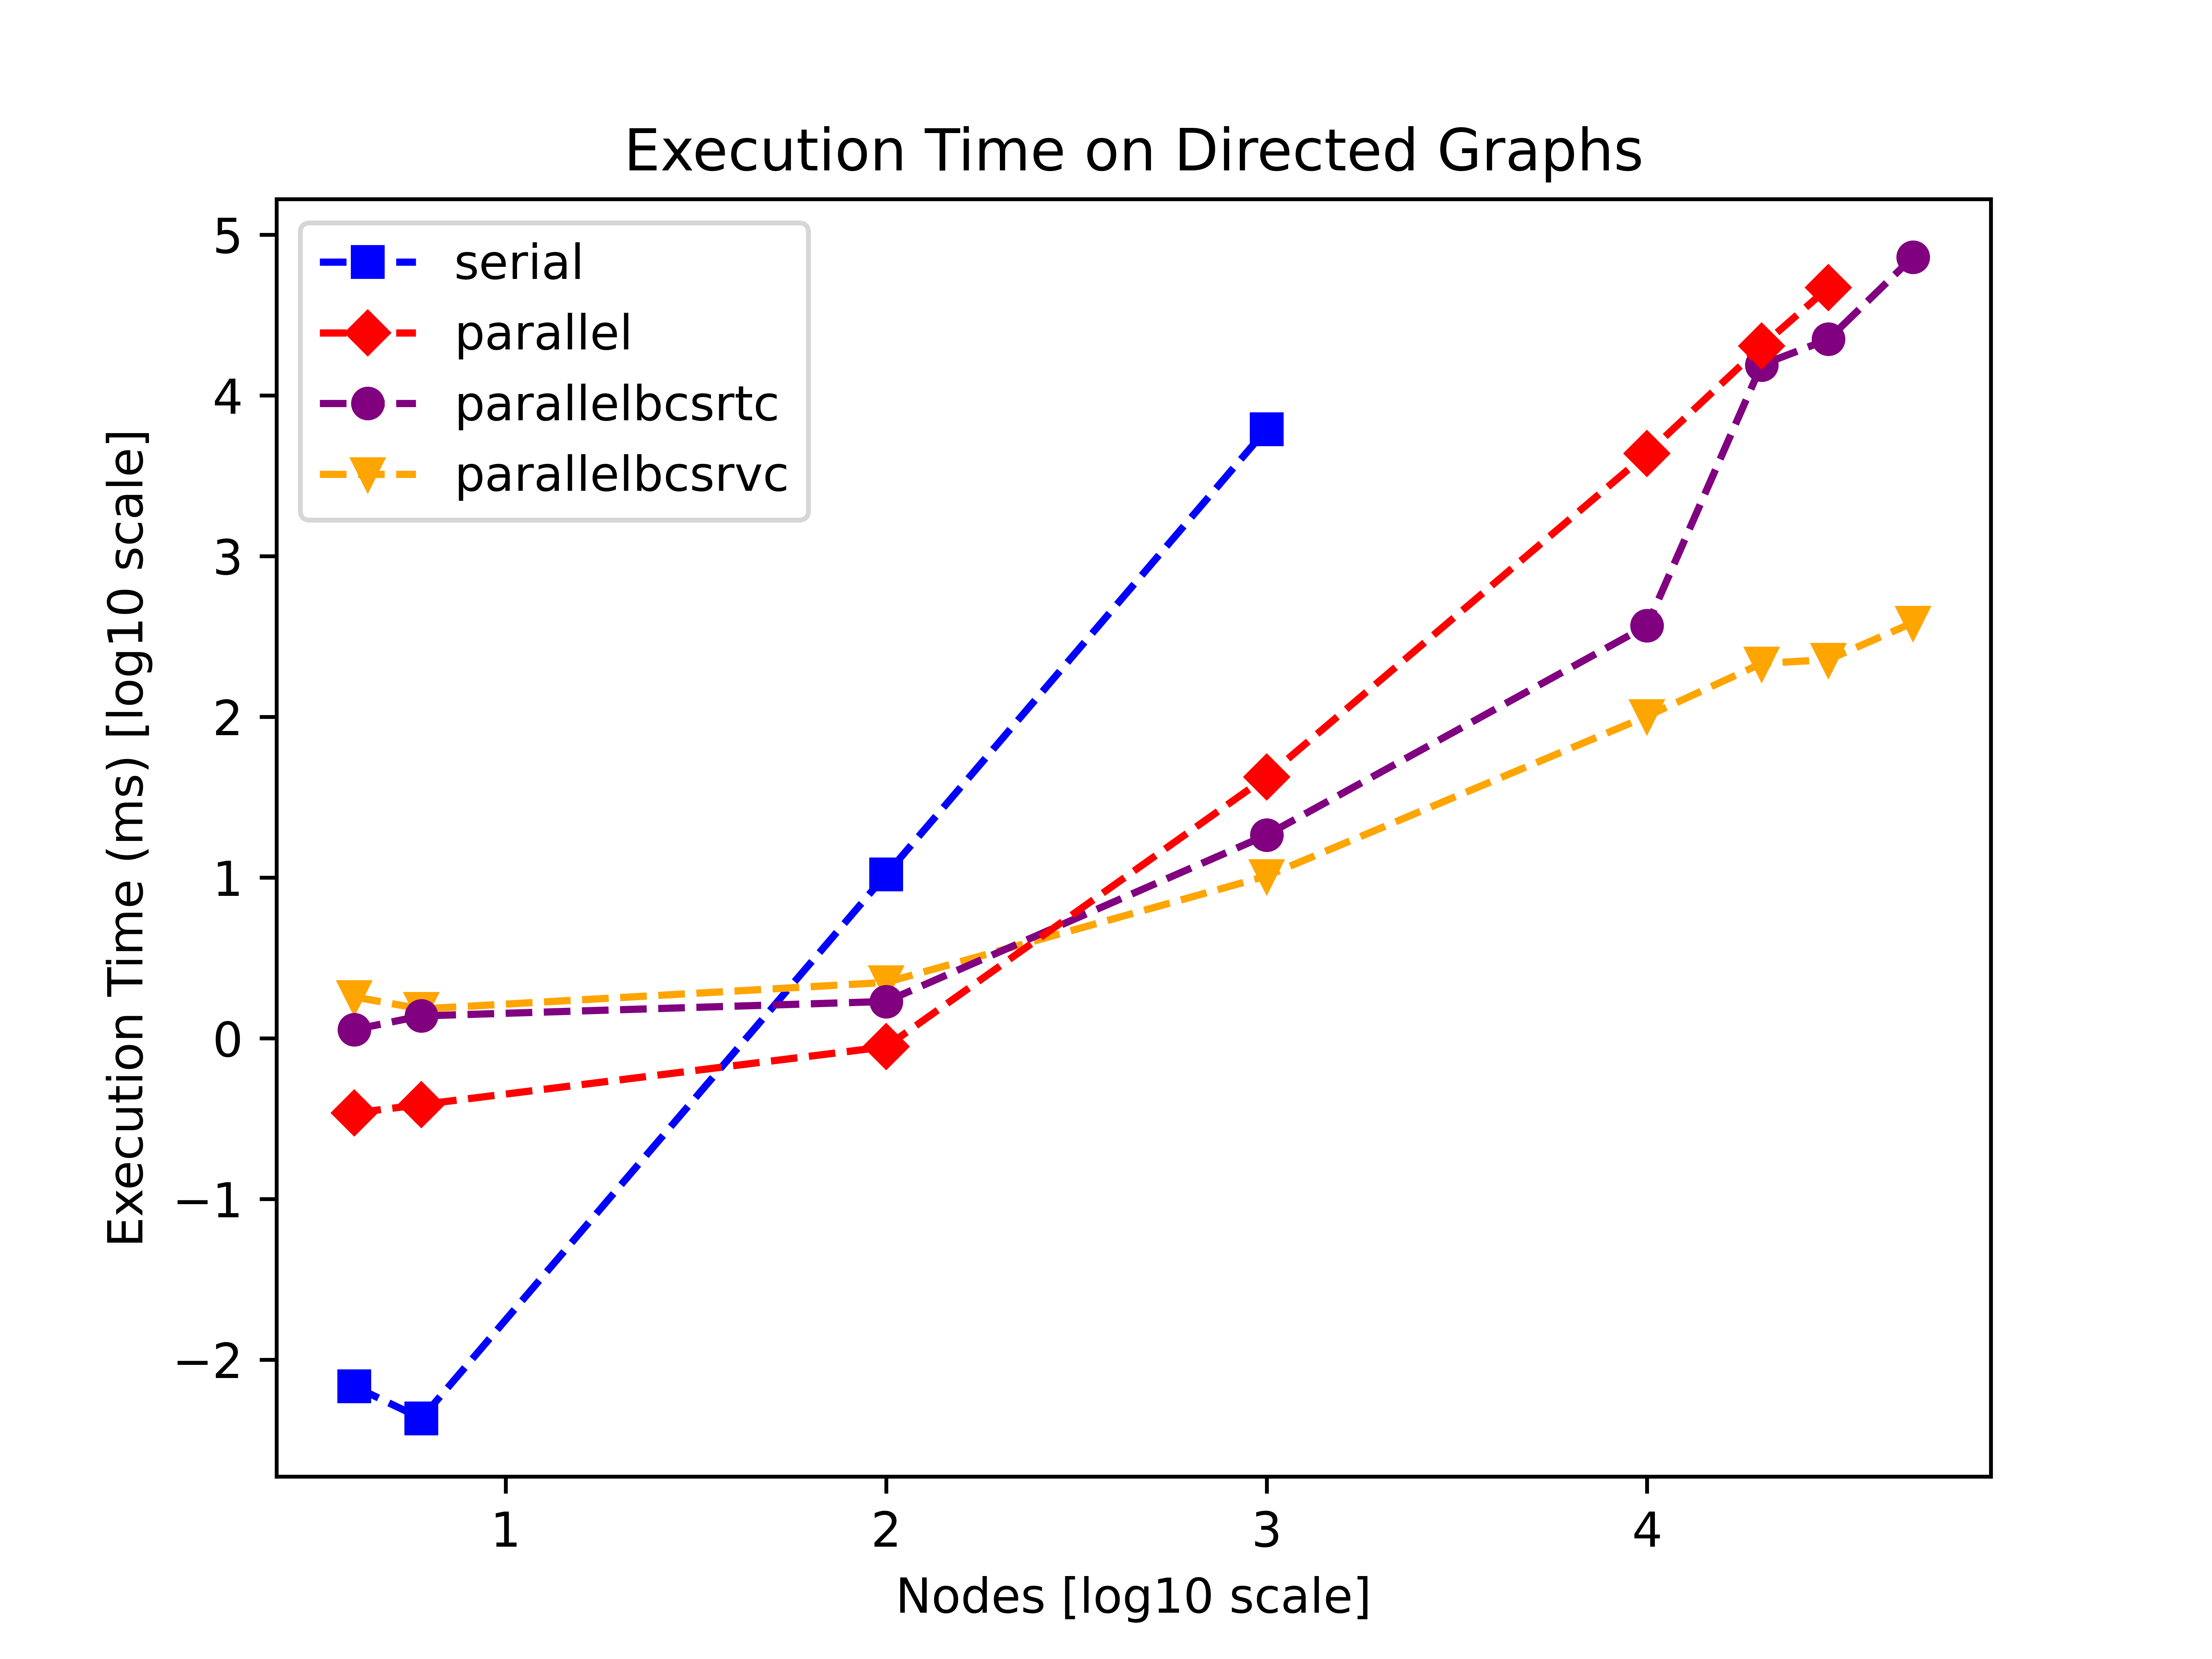
\includegraphics[width=0.7\linewidth]{images/execution_time_directed.png}
        \caption{Tempo di esecuzione dei vari algoritmi con grafi diretti}
        \label{fig:exec-time-dir}
    \end{figure}

    \begin{figure}
        \centering
        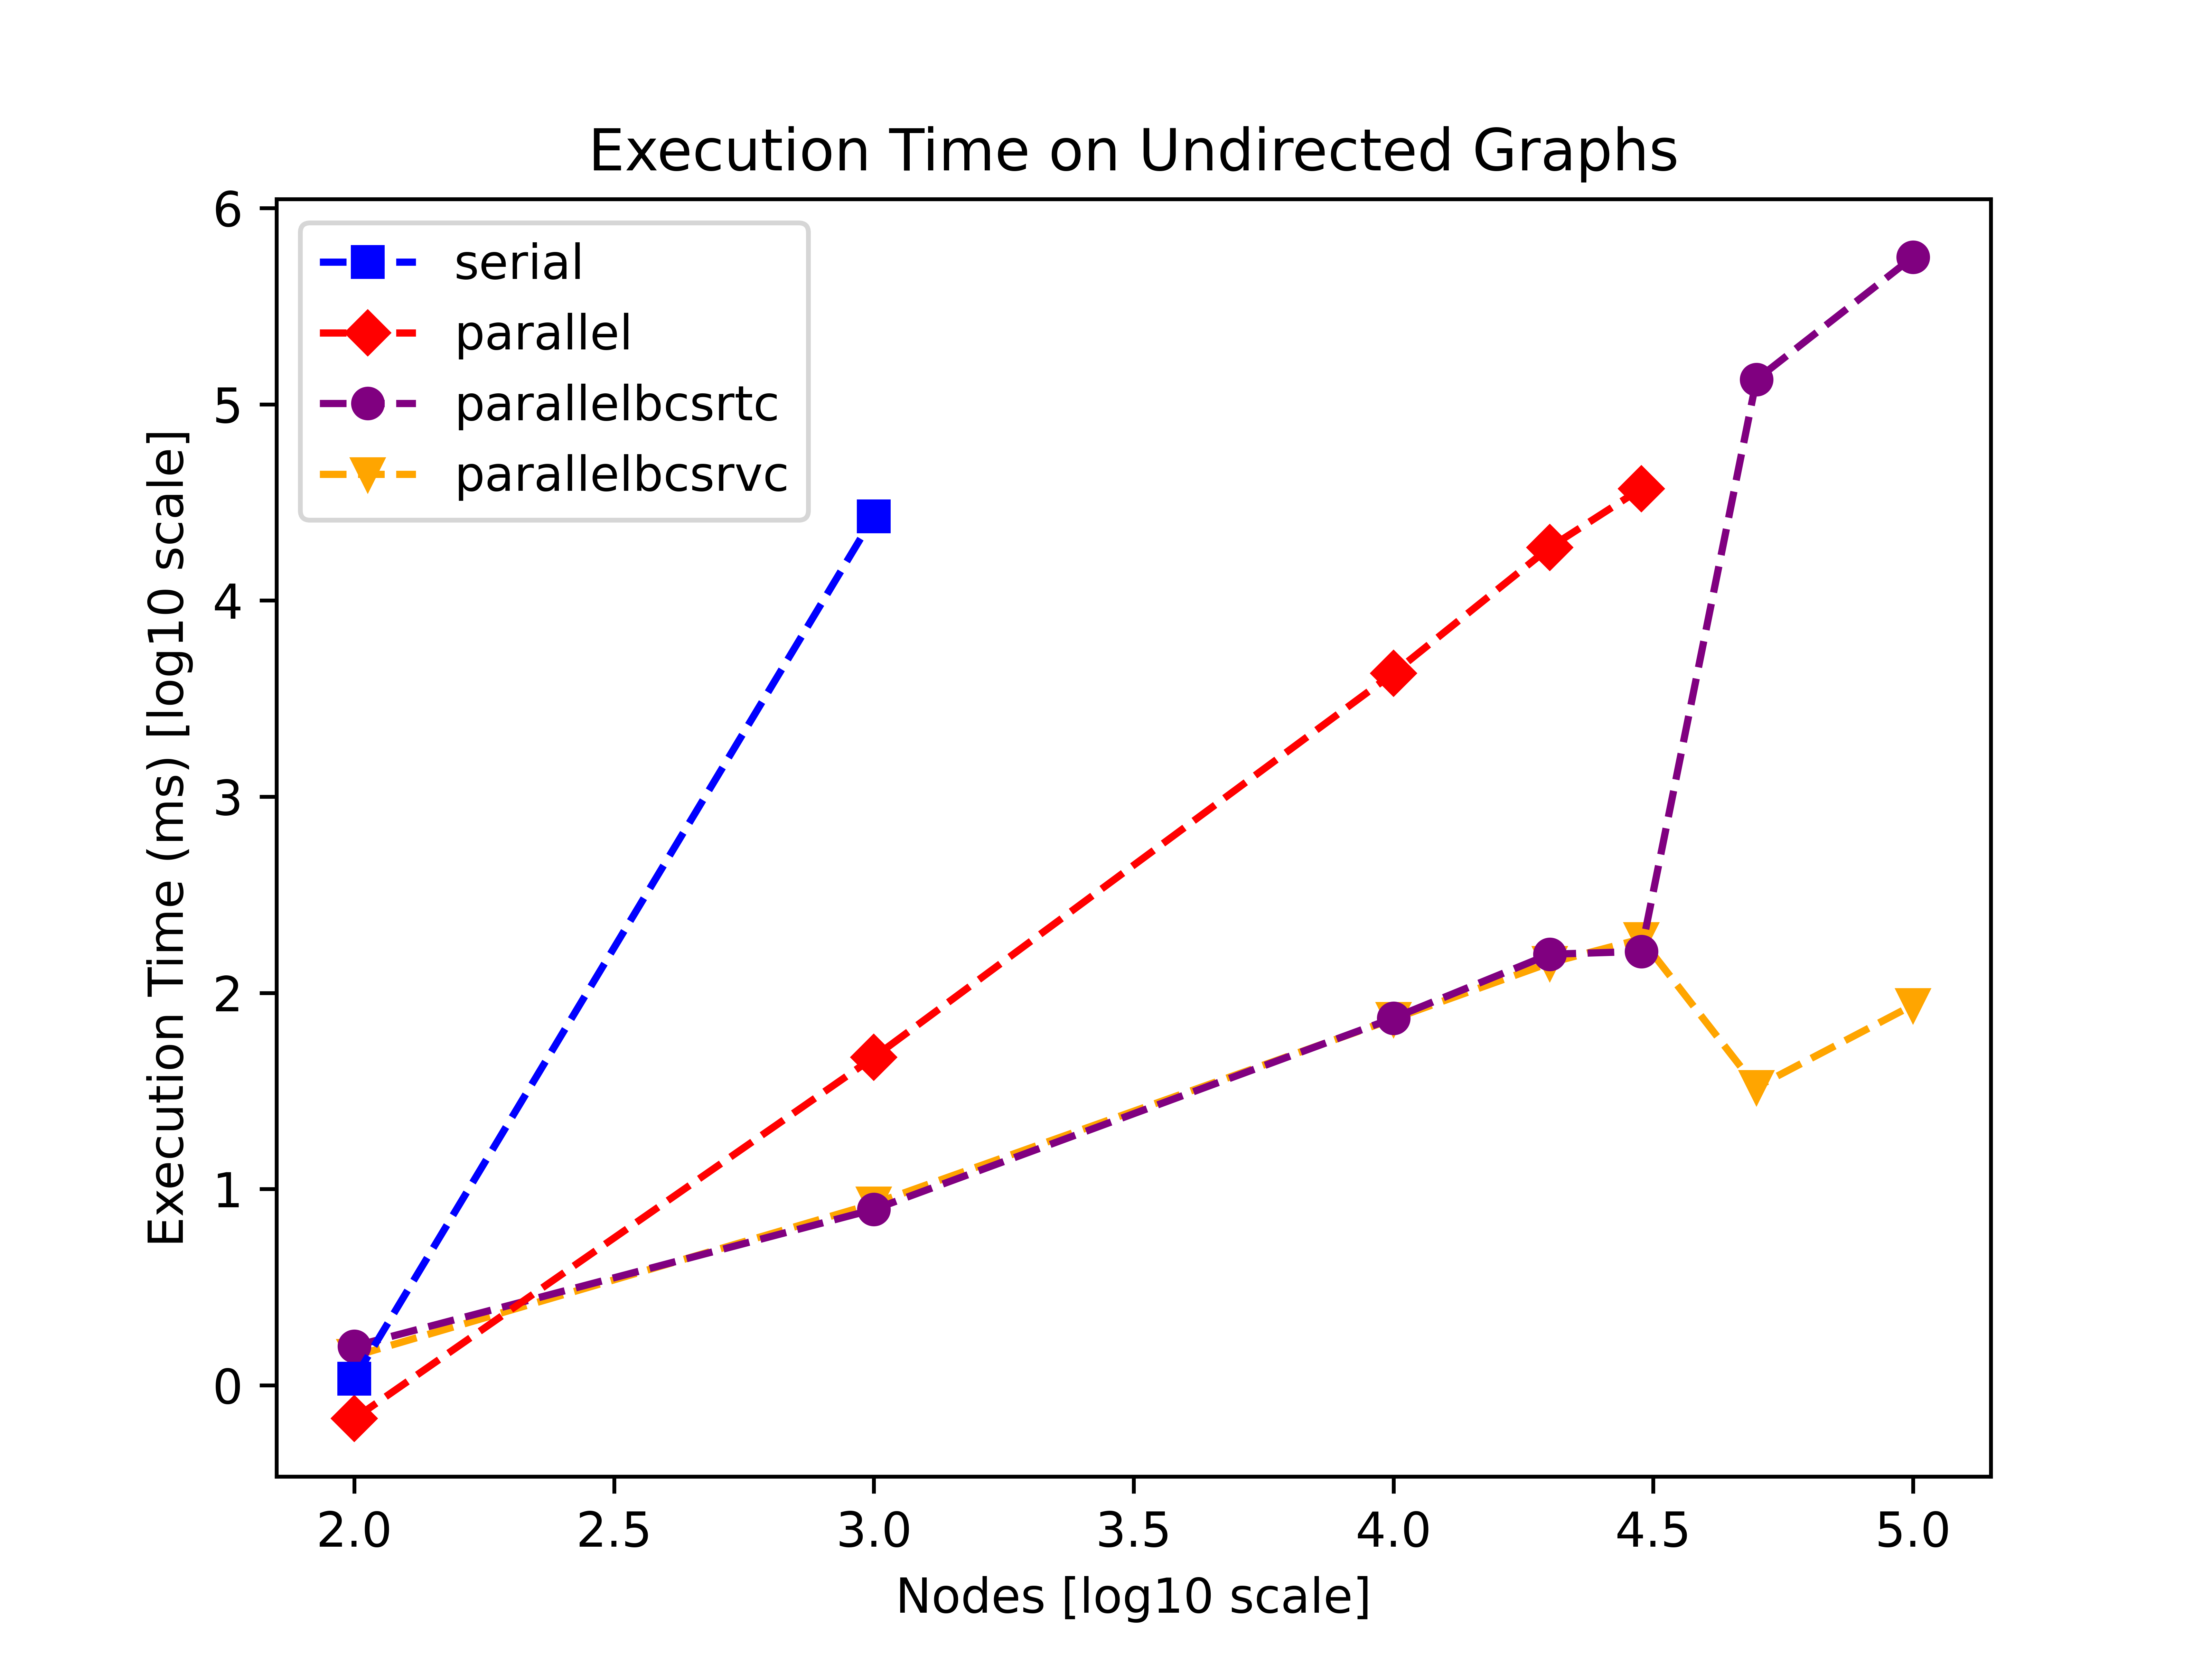
\includegraphics[width=0.7\linewidth]{images/execution_time_undirected.png}
        \caption{Tempo di esecuzione dei vari algoritmi con grafi non diretti}
        \label{fig:exec-time-undir}
    \end{figure}

    \begin{figure}
        \centering
        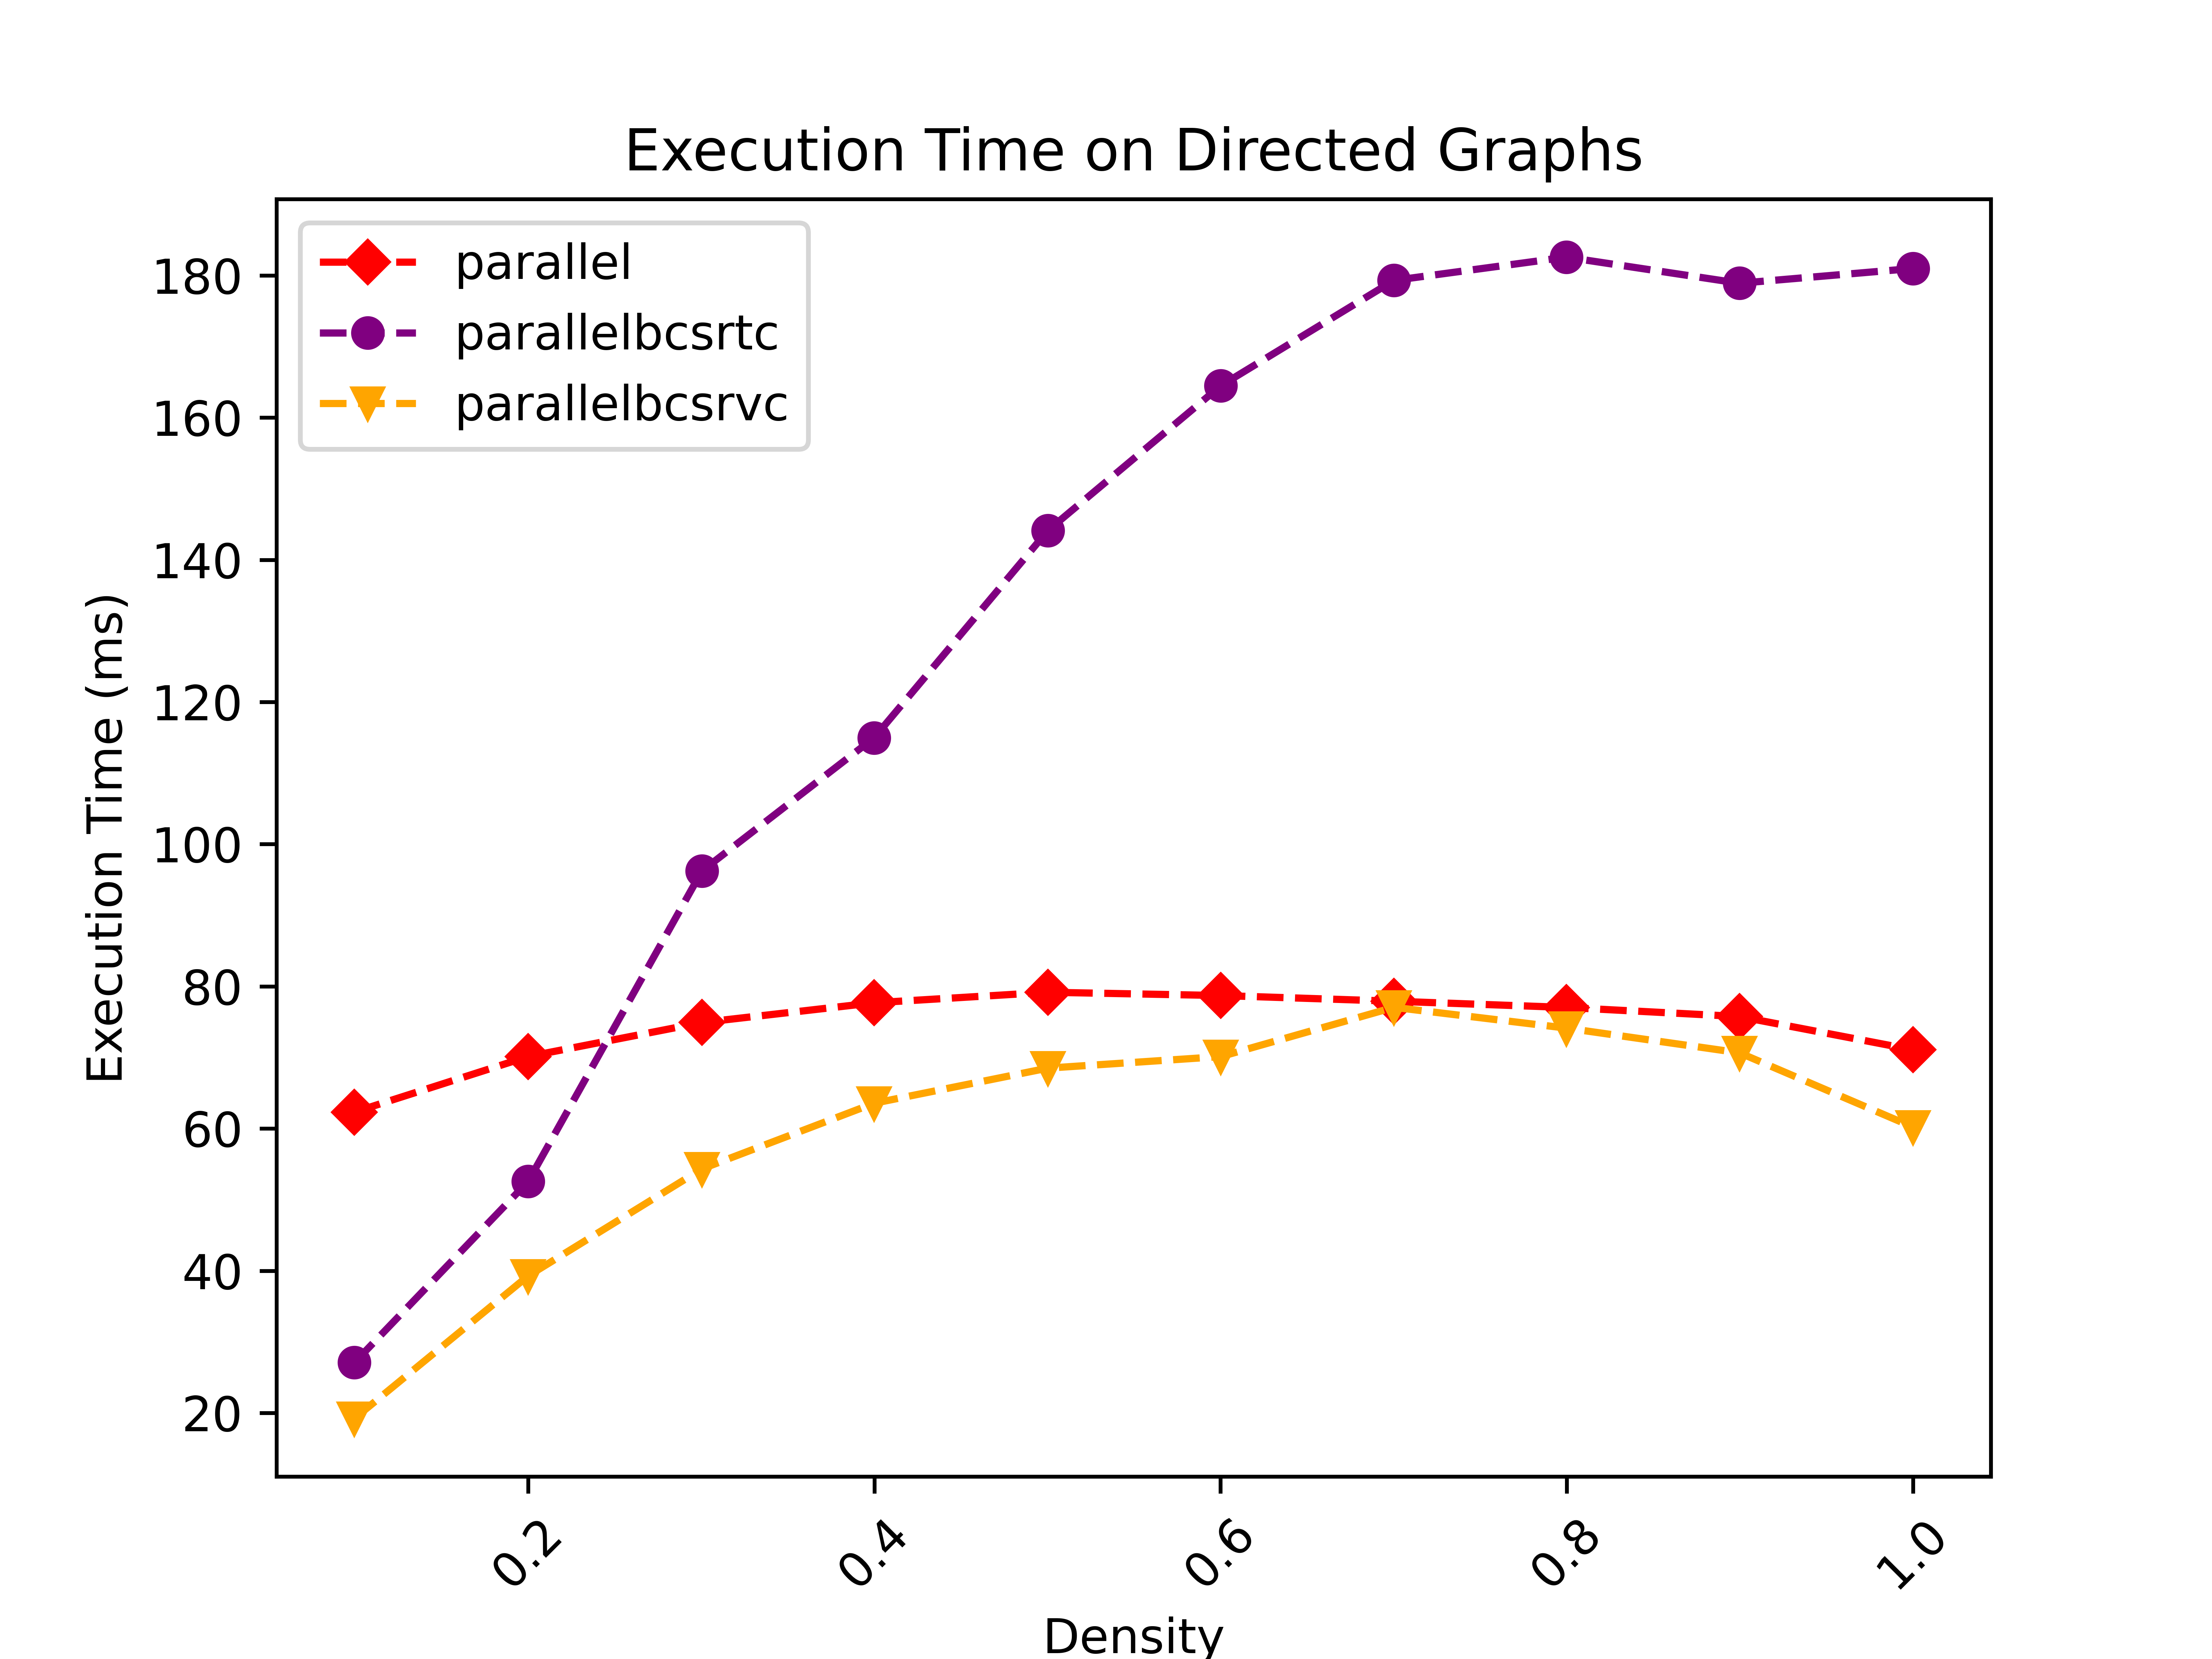
\includegraphics[width=0.7\linewidth]{images/execution_time_density.png}
        \caption{Tempo di esecuzione dei vari algoritmi con grafi diretti a densità variabile}
        \label{fig:exec-time-density}
    \end{figure}





\newpage
Discussione dei risultati
Risultati per test a grafo crescente in numero di nodi
I test eseguiti su grafi con numero di nodi crescente hanno prodotto risultati interessanti, sia per quanto riguarda le versioni parallele dell'algoritmo Push-Relabel applicato a grafi diretti che indiretti.

Grafici di confronto
I grafici di confronto tra le diverse versioni dell'algoritmo mostrano che, all'aumentare del numero di nodi, le prestazioni differiscono notevolmente tra grafi diretti e indiretti.

Grafi diretti: Si osserva che le versioni parallele dell'algoritmo Push-Relabel ottimizzate per grafi diretti tendono a scalare meglio rispetto ai grafi indiretti. Questo comportamento è attribuibile alla struttura delle connessioni nei grafi diretti, che facilita una migliore suddivisione del lavoro tra i thread. Nei grafici, si nota un aumento delle prestazioni fino a un certo numero di nodi, dopo il quale si osserva una stabilizzazione o addirittura un degrado delle prestazioni a causa della crescente complessità delle operazioni di comunicazione e sincronizzazione tra i processori.

Grafi indiretti: Nei grafi indiretti, invece, l'efficienza complessiva è minore. Le versioni parallele ottimizzate per grafi indiretti mostrano un comportamento meno lineare, con una crescita più marcata del tempo di esecuzione all'aumentare del numero di nodi. Questo è probabilmente dovuto alla maggiore interdipendenza tra i nodi nei grafi indiretti, che limita il grado di parallelismo sfruttabile.

Commenti
Per entrambi i tipi di grafo, si osserva un significativo miglioramento delle prestazioni delle versioni parallele rispetto a quelle sequenziali, ma questo beneficio tende a ridursi con l'aumento esponenziale del numero di nodi.
Le prestazioni migliori si ottengono con grafi diretti e un numero medio di nodi, dove il parallelismo è massimizzato senza incorrere in eccessiva latenza dovuta alla sincronizzazione.
Nei grafici di confronto, si osserva che per grafi con un numero di nodi particolarmente elevato, il tempo di esecuzione tende a saturare, evidenziando i limiti intrinseci del parallelismo in presenza di una complessità computazionale crescente.
Risultati per test a grafo con densità crescente
L'esecuzione di test su grafi con densità crescente (numero di archi in proporzione al numero di nodi) ha rivelato alcuni pattern distintivi per quanto riguarda le prestazioni dell'algoritmo Push-Relabel parallelo.

Grafico
Nel grafico che confronta i tempi di esecuzione in funzione della densità del grafo, si osservano due andamenti principali. La matrice di adiacenza con un tempo pressoché costante e la struttura BCSR (Blocked Compressed Sparse Row), che mostra un tempo crescente con la densità.

Osservazioni e possibili spiegazioni
Matrice con tempo costante: L'implementazione dell'algoritmo che utilizza una matrice di adiacenza mantiene tempi di esecuzione pressoché costanti con l'aumentare della densità del grafo. Questo comportamento è dovuto al fatto che, in una matrice, l'accesso ai dati è diretto e non dipende dalla densità del grafo, ma solo dalla dimensione della matrice stessa. Dunque, nonostante un aumento del numero di archi, il tempo necessario per l'accesso e la manipolazione degli elementi non varia significativamente.

BCSR con tempo crescente: Nelle implementazioni che utilizzano la struttura BCSR, si osserva invece un aumento del tempo di esecuzione proporzionale alla densità del grafo. Ciò è spiegabile dal fatto che, con l'aumento della densità, la struttura BCSR diventa progressivamente più complessa e richiede più tempo per la gestione degli archi compressi. In questa struttura, ogni blocco richiede operazioni aggiuntive di lettura e scrittura, il che penalizza le prestazioni quando il numero di archi diventa molto elevato.

Densità elevate, stessi tempi: Un punto interessante evidenziato dai risultati è che, per densità molto elevate, i tempi di esecuzione tendono a convergere tra le varie implementazioni. Questo fenomeno può essere interpretato come un limite superiore intrinseco per entrambe le strutture dati: quando un grafo diventa altamente connesso, i benefici di strutture sparse come BCSR vengono annullati e la complessità complessiva del grafo impatta in maniera uniforme tutte le implementazioni.

Linea viola per BCSR senza ottimizzazioni complete: Nel grafico, si nota una linea viola corrispondente alla versione BCSR non completamente ottimizzata. Questa variante si rivela particolarmente inefficiente e, in definitiva, inutile per grafi con densità elevata, in quanto non riesce a sfruttare adeguatamente le proprietà di compressione della struttura BCSR. Questo risultato conferma che l'ottimizzazione completa delle strutture dati è essenziale per ottenere prestazioni competitive, soprattutto con grafi densi.

Considerazioni finali
I test sui grafi a densità crescente e quelli a numero di nodi crescente forniscono indicazioni complementari sull'efficacia dell'algoritmo Push-Relabel parallelo. Nei grafi a numero di nodi crescente, il parallelismo mostra risultati promettenti ma non senza limitazioni dovute alla complessità della comunicazione tra processi. Nei grafi con densità crescente, invece, l'ottimizzazione delle strutture dati gioca un ruolo determinante nelle prestazioni, specialmente con grafi densi dove strutture come BCSR devono essere attentamente progettate per evitare inefficienze.

In conclusione, le prestazioni dell'algoritmo Push-Relabel parallelo sono fortemente influenzate sia dalla tipologia di grafo che dalle strutture dati utilizzate. La corretta scelta di queste ultime e una buona gestione del parallelismo sono fattori chiave per garantire un'efficace scalabilità dell'algoritmo.

    \chapter{Conclusioni}

    \begin{appendices}

        \chapter{Reti di flusso}\label{app:flownet}

    Formalmente una \textit{rete di flusso} è definita come un grafo orientato $G = (V, E)$ tale che
    \begin{itemize}
        \item Ad ogni arco $(u,v) \in E$ e associato un valore non negativo, $c(u, v) \ge 0$, detto \textit{capacità} dell'arco. Se il nodo $(u, v)$ non è presente in $E$ allora assumiamo che l’arco $(u, v)$ abbia capacità nulla, cioè $c(u, v) = 0$.
        \item Nella rete di flusso ci sono due vertici speciali: il vertice \textit{sorgente} (o \textit{source}), indicato con il simbolo $s$, ed il vertice \textit{pozzo} (o \textit{sink}), indicato con il simbolo $t$.
        \item Ogni vertice giace su qualche cammino dalla sorgente al pozzo. Il grafo è quindi connesso e pertanto vale $|E| \ge |V | - 1$.
    \end{itemize}

    La Figura \ref{fig:flownet} mostra un esempio di rete di flusso. La sorgente ed il pozzo sono rappresentati, rispettivamente, dai simboli $s$ e $t$. Ad ogni arco $(u, v) \in E$ è associato il valore $c(u, v)$.
    
    \begin{figure}[h]
        \centering
        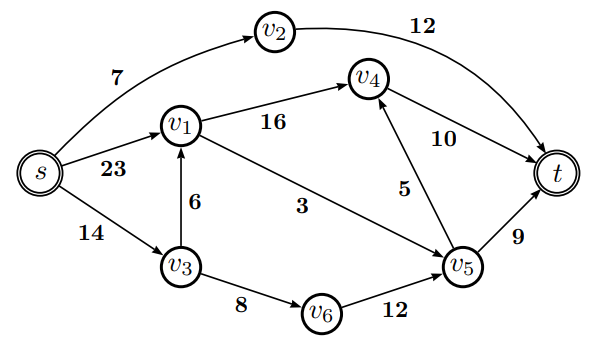
\includegraphics[width=0.6\linewidth]{images/flownet.png}
        \caption{Rete di flusso}
        \label{fig:flownet}
    \end{figure}


    \section{Flusso}

        Per \textit{flusso} in una rete si intende una funzione $x : E \rightarrow \mathbb{R}$ che rispetta i vincoli di capacità del grafo ovvero:
        \begin{equation}
            0 \le x_{ij} \le c(i,j) \quad \forall (i,j) \in E
        \end{equation}

        Con il termine \textit{divergenza} di un nodo $i$ si intende la differenza tra il flusso uscente e quello entrante ovvero, dato un nodo $v \in V$ e un flusso $x$ in $G$:
        \begin{equation}
            \Delta_x(v) = \sum_{\mathclap{\substack{j \in V \\ (v,j) \in E}}}x_{vj} - \sum_{\mathclap{\substack{i \in V \\ (i,v) \in E}}}x_{iv}
        \end{equation}

        Si dice che il flusso $x$ è conservato nel nodo $v$ (o che il flusso $x$ soddisfa i vincoli di conservazione del flusso) se $\Delta_x(v) = 0$. Un flusso che è conservato per ogni nodo è detto \textit{circolazione}. Una \textit{circolazione} può essere vista come uno scambio di beni in cui nulla viene mai creato o distrutto, ma è semplicemente passato da un nodo all'altro.

        Se un flusso non è una circolazione, assumendo $S:=\{v : \Delta_x(v) > 0 \}$ e $T:=\{v : \Delta_x(v) < 0 \}$, possiamo interpretare il flusso come uno spostamento di beni in quantità $\phi = \sum_{v \in S} \Delta_x(v)$ dai nodi in $S$ a quelli in $T$. Infatti, tutto il flusso uscente da $S$ entrerà nei nodi in $T$.

        Se consideriamo $s$ (source) e $t$ (sink) due nodi distinti in $V$, ogni flusso che è conservato in ogni nodo $v \neq s,t$ è chiamato \textit{flusso s-t} e il suo valore è definito come:
        \begin{equation}
            \phi_x = \Delta_x(s)
        \end{equation}

        Il problema del trovare il flusso s-t con valore massimo (dati $s$ e $t$) all'interno di una rete è chiamato \textit{problema del massimo flusso} \cite{Lancia2022}.
        
    \section{Rete residua}
        Sia $f$ un flusso in una rete (G, c), e si consideri una coppia di vertici $u, v \in V$ . La quantità di flusso che possiamo inviare da $u$ a $v$ prima di superare la capacità $c(u, v)$ è la \textit{capacità residua} di $(u, v)$, ed è data da 
        \begin{equation}
            c_f (u, v) = c(u, v) - f(u, v)
        \end{equation}

        Data una rete di flusso $(G, c)$ ed un flusso $f$, la rete residua di $G$ indotta da $f$ è $G_f = (V, E_f )$, dove
        \begin{equation}
            E_f = \{(u, v) \in V \times V : c_f(u, v) > 0\}
        \end{equation}
        
        Ogni arco della rete, chiamato \textit{arco residuo}, può ammettere un flusso strettamente positivo.
        Un arco $(u, v)$ può essere un arco residuo in $E_f$ , anche se esso non fosse un arco in $E$, ma purché $(v, u) \in E$. Ciò implica che non sempre vale la relazione $E_f \subseteq E$. Però si ha sempre
        \begin{equation}
            |E_f| \le 2 \cdot |E|
        \end{equation}
        
        Si osservi che la rete residua $G_f$ è essa stessa una rete di flusso avente capacità definita dalla funzione $c_f$.
    

        \chapter{Tecniche di Rappresentazione di Grafi}\label{app:csr}

    In questo capitolo sono descritte due delle principali tecniche utilizzate per rappresentare i grafi: la rappresentazione a matrice di adiacenza e la rappresentazione \textit{Compressed Sparse Row}.

    \section{Rappresentazione dei Grafi con Matrici di Adiacenza}
        Una matrice di adiacenza è una rappresentazione comunemente utilizzata per descrivere un grafo $G = (V, E)$, dove $V$ è l'insieme dei vertici e $E$ è l'insieme degli archi (o collegamenti) tra i vertici. Questa tecnica rappresenta il grafo come una matrice quadrata di dimensioni $|V| \times |V|$, con le seguenti caratteristiche:

        \begin{itemize}
            \item ogni riga e colonna della matrice corrisponde a un vertice del grafo;
            \item il valore in posizione $(i, j)$ della matrice indica se esiste un arco tra il vertice $i$ e il vertice $j$;
            \item per grafi non pesati, l'elemento $A[i][j]$ è uguale a 1 se esiste un arco tra $i$ e $j$, altrimenti è uguale a 0;
            \item per grafi pesati, l'elemento $A[i][j]$ contiene il peso dell'arco tra $i$ e $j$ (se esiste), mentre un valore predefinito, come $\infty$ o 0, è usato per indicare l'assenza di un arco;
            \item per grafi non orientati, la matrice di adiacenza è simmetrica rispetto alla diagonale principale, poiché un arco tra $i$ e $j$ implica anche un arco tra $j$ e $i$.
        \end{itemize}
    
        Questo tipo di rappresentazione è particolarmente utile per grafi densi, dove la maggior parte dei vertici sono connessi tra loro, poiché richiede $O(|V|^2)$ spazio di memoria.
    
        La matrice di adiacenza offre un modo semplice e diretto per eseguire operazioni come la verifica dell'esistenza di un arco tra due vertici, con una complessità $O(1)$. Tuttavia, può diventare inefficiente in termini di spazio di memoria per grafi molto sparsi, dove il numero di archi è significativamente inferiore a $|V|^2$. In questi casi, altre tecniche di rappresentazione, come le liste di adiacenza o il formato CSR per matrici sparse, possono essere più appropriate.


    \section{Compressed Sparse Row}
    
        Una matrice sparsa memorizzata in formato CSR (\textit{Compressed Sparse Row}) è una rappresentazione compatta che si basa sul memorizzare solo gli elementi non nulli della matrice. Questa tecnica è particolarmente utile per matrici sparse di grandi dimensioni, dove la maggior parte degli elementi è zero, riducendo drasticamente lo spazio di memoria richiesto rispetto alla memorizzazione di una matrice completa. Nel formato CSR, la matrice è rappresentata dai seguenti parametri:
    
        \begin{itemize}
            \item il numero di righe nella matrice;
            \item il numero di colonne nella matrice;
            \item il numero di elementi non nulli (\textit{nnz}) nella matrice;
            \item i puntatori all'array degli offset delle righe, di lunghezza pari al numero di righe $+ 1$, che rappresentano la posizione iniziale di ciascuna riga negli array delle colonne e dei valori;
            \item i puntatori all'array degli indici delle colonne, di lunghezza \textit{nnz}, che contiene gli indici delle colonne degli elementi corrispondenti nell'array dei valori;
            \item i puntatori all'array dei valori, di lunghezza \textit{nnz}, che contiene tutti i valori non nulli della matrice, ordinati in base alle righe.
        \end{itemize}

        La rappresentazione CSR permette di effettuare operazioni come il prodotto matrice-vettore in modo più efficiente, poiché si evita di processare esplicitamente gli elementi nulli. Inoltre, poiché gli elementi non nulli sono memorizzati in forma compatta, si riduce notevolmente il consumo di memoria \cite{NvidiaWebsite}.
        
        La Figura \ref{fig:graph-example} mostra un grafo orientato con 5 vertici mentre la Figura \ref{fig:csr-example} mostra come la rete si possa rappresentare secondo le due tecniche appena viste.
        
        \begin{figure}[h]
            \centering
            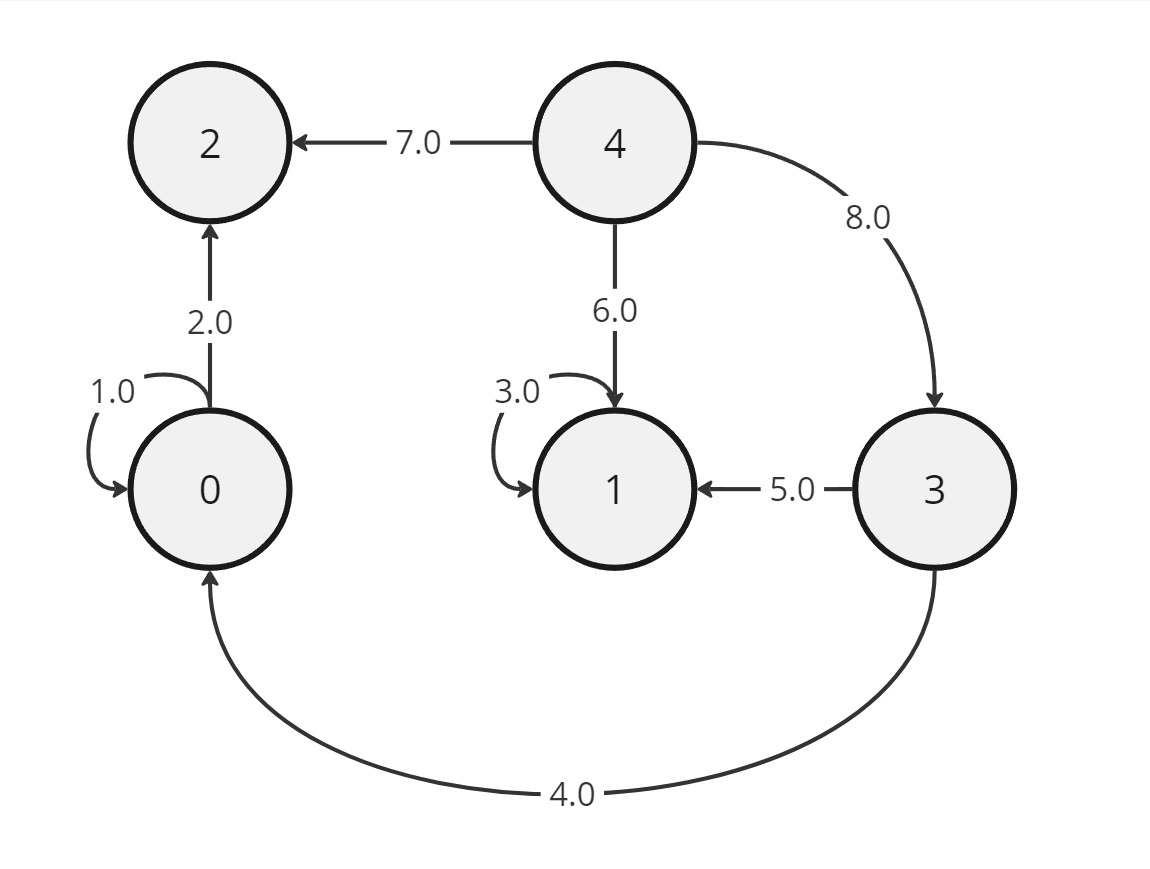
\includegraphics[width=0.5\linewidth]{images/graph.jpg}
            \caption{Esempio di grafo diretto pesato}
            \label{fig:graph-example}
        \end{figure}

        \begin{figure}[h]
            \centering
            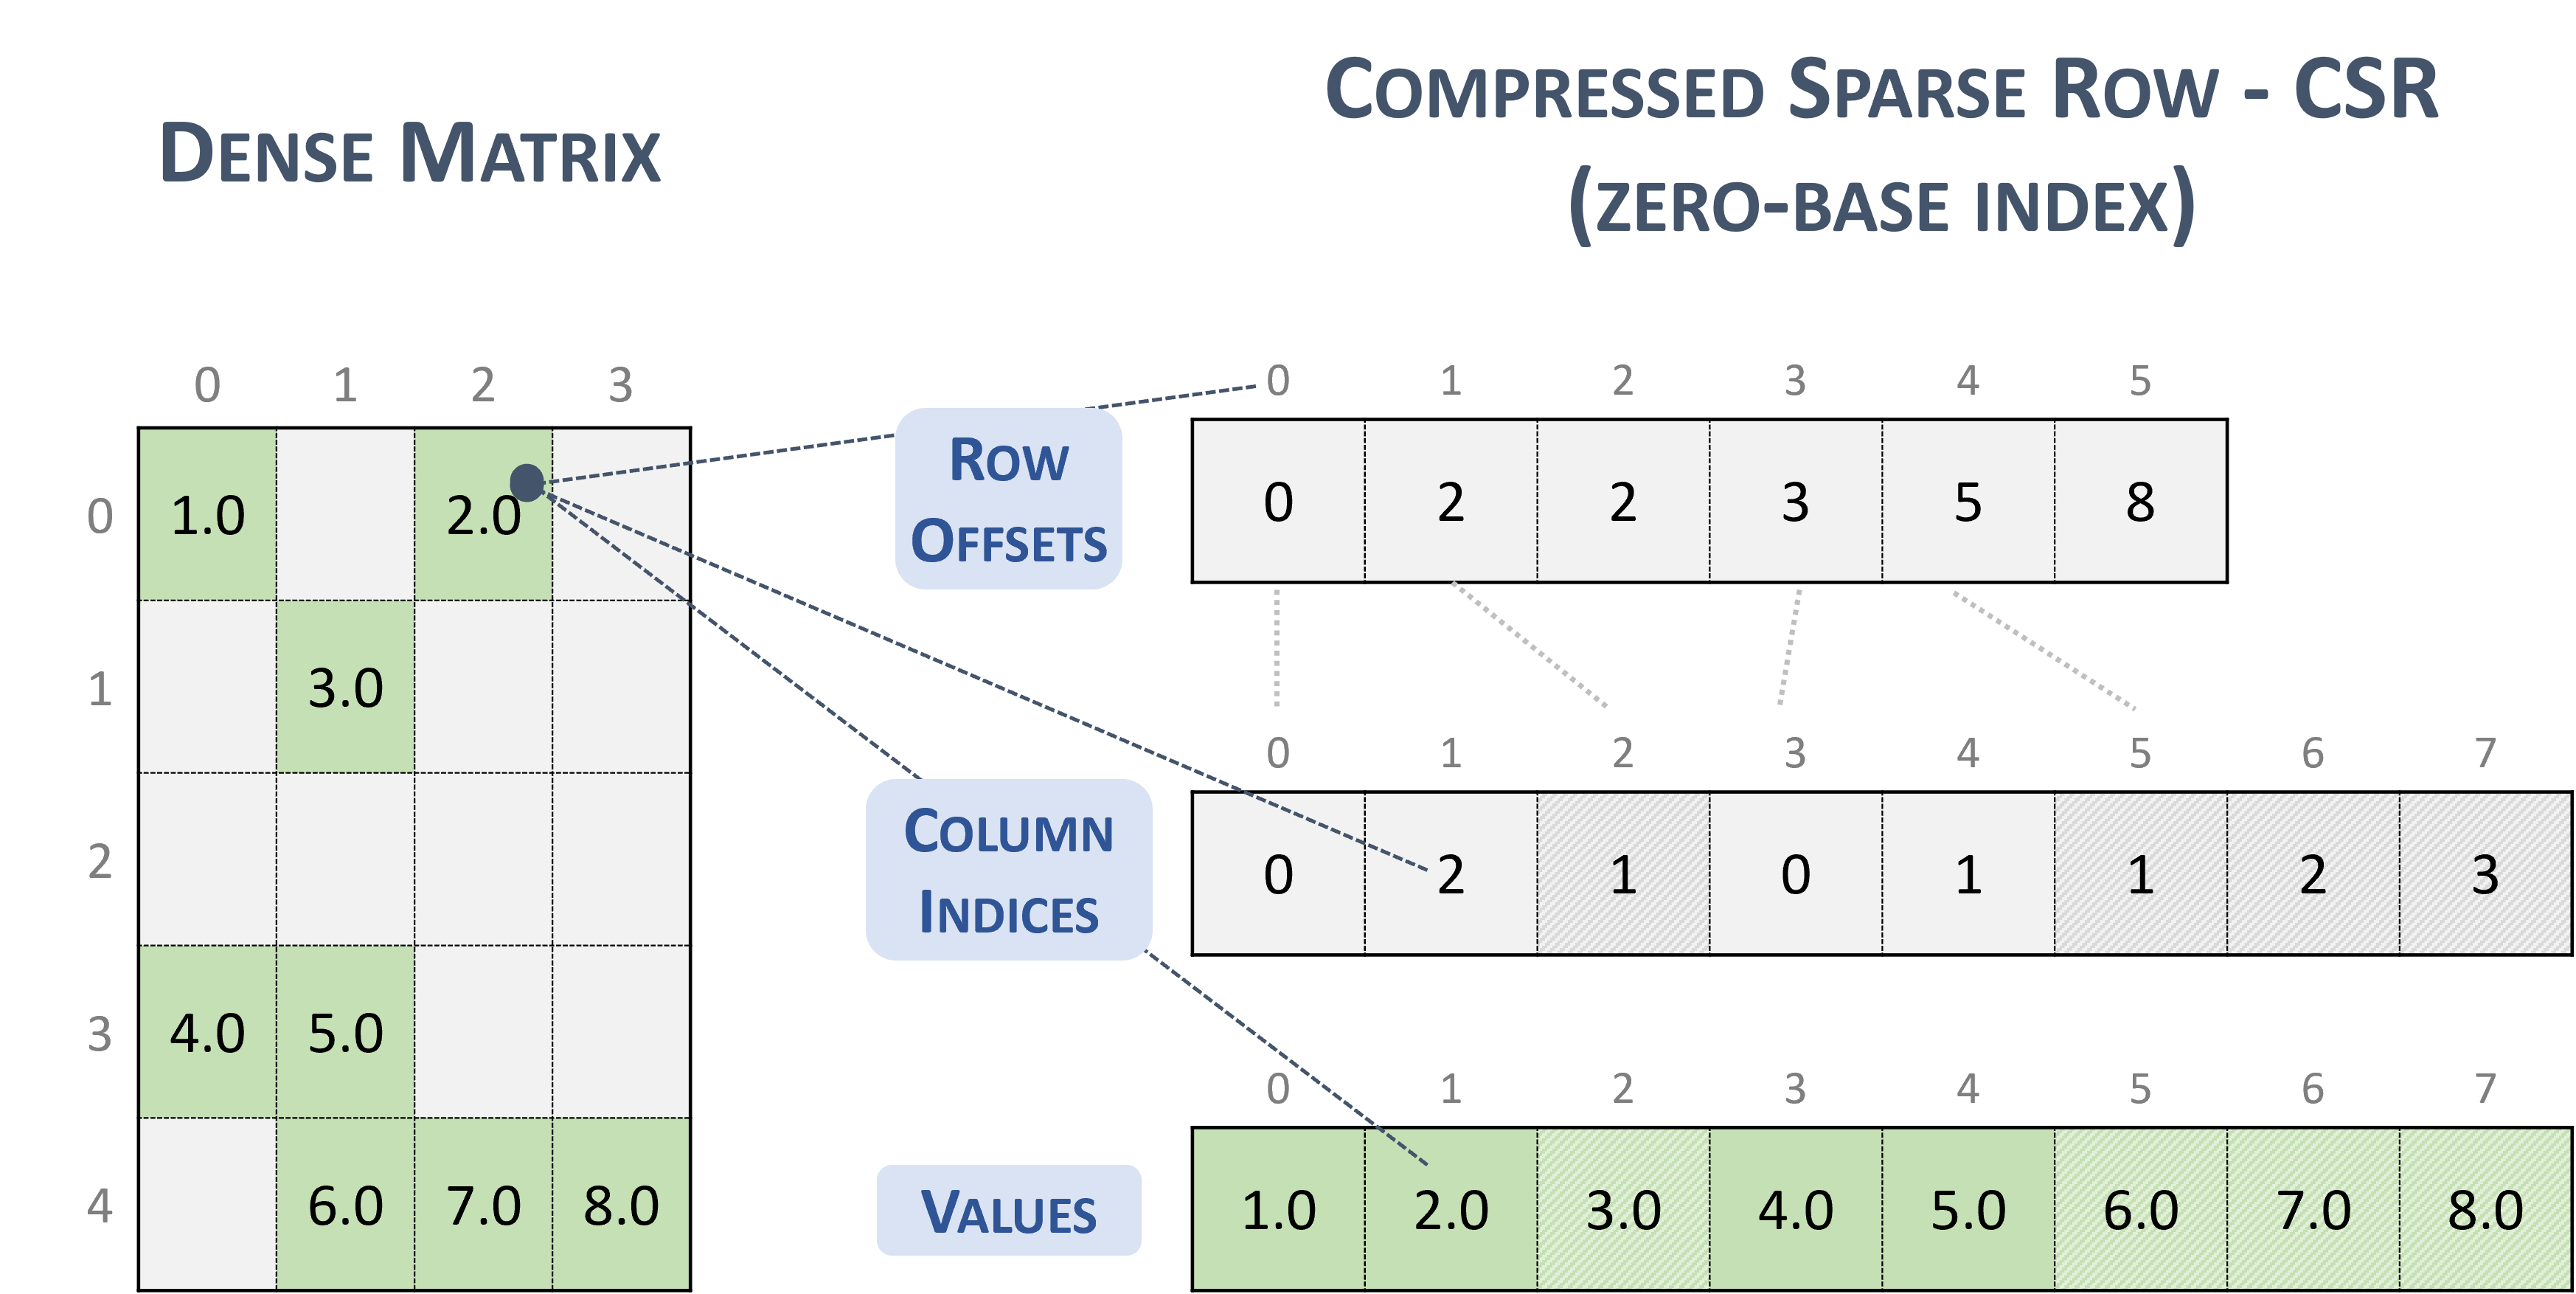
\includegraphics[width=0.9\linewidth]{images/csr-example.png}
            \caption{Matrice di adiacenza vs CSR}
            \label{fig:csr-example}
        \end{figure}


		\chapter{Guida all'uso}\label{app:guida}

    \subsubsection*{Struttura del progetto}

        Ogni implementazione è contenuta all'interndo di una cartella. 
        \begin{description}
            \item[\texttt{serial}] contiene l'implementazione seriale dell'algoritmo Push-Relabel;
            \item[\texttt{parallel}] contiene la prima implementazione parallela basata sulla matrice di adiacenza;
            \item[\texttt{parallel\_bcsr\_tc}] contiene la seconda implementazione parallela basata sulla rappresentazione BCSR;
            \item[\texttt{parallel\_bcsr\_vc}] contiene la terza implementazione parallela basata sulla rappresentazione BCSR e ottimizzata per bilanciare il lavoro tra i vari thread della GPU.  
        \end{description}

        Il contenuto di ogni cartella è il seguente:
        \begin{itemize}
            \item cartella \texttt{include} contenente i file header;
            \item cartella \texttt{src} contenente i file sorgente;
            \item file \texttt{main.cpp} o \texttt{main.cu} contenente il main del programma;
            \item due script per eseguire i test al variare del numero di nodi e della densità del grafo. 
        \end{itemize}


    \subsubsection*{Compilazione ed esecuzione}

        All'esterno delle cartelle è presente un unico \texttt{Makefile} per compilare il codice sorgente delle diverse implementazioni e per eseguire gli script di test. 
        In particolare, per la compilazione sono disponibili i seguenti comandi:
        \begin{description}
            \item[\texttt{make all}] compila il codice sorgente di tutte le implementazioni;
            \item[\texttt{make prserial}] compila il codice sorgente dell'implementazione seriale;
            \item[\texttt{make prparallel}] compila il codice sorgente dell'implementazione parallela basata sulla matrice di adiacenza;
            \item[\texttt{make prparallelbcsrtc}] compila il codice sorgente dell'implementazione parallela basata sulla rappresentazione BCSR;
            \item[\texttt{make prparallelbcsrvc}] compila il codice sorgente dell'implementazione parallela basata sulla rappresentazione BCSR e ottimizzata per bilanciare il lavoro tra i vari thread della GPU;
        \end{description}

        Una volta ottenuti i file eseguibili, è possibile eseguire il programma lanciando il comando \verb|[path eseguibile] [path file input] [path file output] [flag calcolo mincut]| facendo attenzione ai seguenti aspetti:
        \begin{itemize}
            \item il file di input deve essere un file di testo con estensione \verb|.txt| o \verb|.max| contenente la rappresentazione del grafo secondo uno dei formati descritti nella sezione \ref{sec:input-data};
            \item se nel percorso del file di output sono presenti delle directory, queste devono essere già esistenti;
            \item al nome del file verrà aggiunto un timestamp per evitare sovrascritture;
            \item il flag per il calcolo del mincut è opzionale e può essere 0 o 1; se non specificato, il programma calcolerà il mincut.
        \end{itemize}

        Un esempio di comando per l'esecuzione è il seguente:

        \verb|./serial/prserial input_data/graph1.txt results/graph1_serial_results.json 0|


    \subsubsection*{Esecuzione script di test}

        Per eseguire gli script di test sono disponibili i seguenti comandi:
        \begin{description}
            \item[\texttt{make test}] esegue gli script di test per le diverse implementazioni al variare del numero di nodi;
            \item[\texttt{make testdensity}] esegue gli script di test per le diverse implementazioni al variare della densità del grafo;
            \item[\texttt{make testserial}] esegue gli script di test per l'implementazione seriale al variare del numero di nodi;
            \item[\texttt{make testparallel}] esegue gli script di test per l'implementazione parallela basata sulla matrice di adiacenza al variare del numero di nodi;
            \item[\texttt{make testparallelbcsrtc}] esegue gli script di test per l'implementazione parallela basata sulla rappresentazione BCSR al variare del numero di nodi;
            \item[\texttt{make testparallelbcsrvc}] esegue gli script di test per l'implementazione parallela basata sulla rappresentazione BCSR e ottimizzata per bilanciare il lavoro tra i vari thread della GPU al variare del numero di nodi;
            \item[\texttt{make testdensityparallel}] esegue gli script di test per l'implementazione parallela basata sulla matrice di adiacenza al variare della densità del grafo;
            \item[\texttt{make testdensityparallelbcsrtc}] esegue gli script di test per l'implementazione parallela basata sulla rappresentazione BCSR al variare della densità del grafo;
            \item[\texttt{make testdensityparallelbcsrvc}] esegue gli script di test per l'implementazione parallela basata sulla rappresentazione BCSR e ottimizzata per bilanciare il lavoro tra i vari thread della GPU al variare della densità del grafo;
        \end{description}

        A qualsiasi comando tra quelli sopra elencati è possibile aggiungere l'opzione \texttt{n=[numero]} per specificare il numero di volte che si vuole eseguire ogni singolo test. Ad esempio, il comando \texttt{make testdensityparallel n=10} eseguirà lo script \verb|parallel/testdensityparallel.sh| 10 volte.

        I risultati dei test vengono salvati in file JSON all'interno della cartella \texttt{results}.


    \subsubsection*{Altri comandi}

        Infine, sono disponibili i seguenti comandi per la pulizia dei file generati:
        \begin{description}
            \item[\texttt{make clean}] elimina i file oggetto e gli eseguibili generati dalla compilazione;
            \item[\texttt{make cleanallresults}] elimina i file contenenti i risultati dei test dalla directory \texttt{results}.
        \end{description}

        Ulteriori comandi per la pulizia dei file dei risultati sono disponibili all'interno del Makefile.


    \end{appendices}

    % Creazione sezione riferimenti
    \printbibliography[title=Riferimenti]
    
\end{document}